\chapter{Implementácia mobilnej aplikácie vo frameworku Flutter}
\label{chap:implementacia}
Táto kapitola opisuje konkrétnu realizáciu aplikácie Office Hours vo frameworku Flutter. Nadväzuje na kapitoly~\ref{chap:analyza} a~\ref{chap:navrh} a ukazuje, ako boli požiadavky a návrh používateľského rozhrania a architektúry implementované.

\section{Prehľad projektu a adresárová štruktúra}
\label{sec:impl-struktura}

Celý zdrojový kód klientskej aplikácie sa nachádza v priečinku \textbf{lib/}.
Vstupným bodom aplikácie je súbor \textbf{main.dart}. Súbor \textbf{setup.dart} centralizuje globálne
inštancie služieb (navigátor, správca relácie, notifikácie a pod.)
dostupné v celej aplikácii. Adresárová štruktúra priečinka \textbf{lib/} priamo odráža
architektonický vzor MVVM popísaný v kapitole~\ref{chap:technologie}. Celková štruktúra projektu
je uvedená v prílohe~\ref{priloha-struktura}.
Konvencie pomenovania súborov sú popísané v sekcii~\ref{subsec:strukturanavrh}.

\section{Architektúra MVVM v praxi}
\label{sec:impl-mvvm}
V tejto sekcii je popísané, ako je architektonický vzor MVVM z kapitoly~\ref{chap:technologie} implementovaný v konkrétnych triedach aplikácie.

\subsection{Dátové modely a JSON konverzia}
Na to, aby aplikácia dokázala efektívne pracovať
s dátami prijímanými z REST API vo formáte JSON, bolo potrebné navrhnúť
silne typované klientske dátové modely. Každý model implementuje metódu fromJson na konverziu JSON odpovede na typovanú inštanciu triedy.

Aplikácia pracuje so štyrmi modelmi, ktoré odrážajú štruktúru dát na serveri:

\begin{itemize}
    \item \textbf{UserModel}: Reprezentuje informácie o prihlásenom používateľovi, vrátane jeho mena, priezviska, roly (učiteľ/študent) a e-mailovej adresy.
    \item \textbf{RoomModel}: Reprezentuje konzultačnú miestnosť.
    Okrem iného obsahuje názov,
    voliteľný popis – typicky fyzická poloha
    miestnosti na fakulte, napríklad \textit{„L224"} – a pole
    \textbf{link}, ktoré uchováva externý odkaz
    priradený k miestnosti, napríklad link na online konzultácie alebo
    osobnú stránku vyučujúceho. Model ďalej obsahuje zoznam e-mailových adries a domén, ktorým Majiteľ povolil prístup do miestnosti.
    \item \textbf{BlockModel}: Definuje časový blok viazaný na
    konkrétnu miestnosť. Obsahuje napríklad dátum konania,
    voliteľnú poznámku, príznak
    online konania a zoznam inštancií
    \textbf{SlotModel}.
     \item \textbf{SlotModel}: Predstavuje konkrétny rezervovateľný termín. Obsahuje čas začiatku,
    trvanie v minútach, príznak online konania a pole \textbf{takenBy} (ak je slot voľný,
    hodnota je \textbf{null}, ak je obsadený, obsahuje identifikátor
    používateľa, ktorý si ho rezervoval) a rôzne ďalšie.
\end{itemize}

\subsection{Obrazovky a komponenty}

Každá obrazovka aplikácie je implementovaná ako samostatný
\textbf{StatefulWidget} alebo \textbf{StatelessWidget}, ktorý zodpovedá
jednému súboru \textbf{*\_page.dart}. Prezentačná vrstva je od logiky oddelená
prostredníctvom balíčka \textbf{provider} v súlade s architektonickým vzorom
MVVM popísaným v kapitole~\ref{chap:technologie}: každá obrazovka obaľuje telo
widgetom \textbf{ChangeNotifierProvider} a reaktívne vykresľovanie zabezpečuje
\textbf{Consumer<T>}.

Rozlišujú sa dva spôsoby poskytnutia ViewModelu. Ak obrazovka ViewModel vytvára a vlastní, použije sa \textbf{ChangeNotifierProvider(create: \_)} a životný cyklus inštancie je viazaný na životný cyklus daného \textbf{State}. Príkladom je \textbf{RegistrationPage} alebo \textbf{EmailInputPage}. Ak naopak ViewModel vznikol mimo stromu widgetov – napríklad v metóde \textbf{initState()}, použije sa variant \textbf{ChangeNotifierProvider.value}, ktorý inštanciu iba sprístupní bez toho, aby ju po zrušení widgetu zničil. Tento prístup je uplatnený napríklad v \textbf{ConsultationsOwnerPage} alebo \textbf{DisplaySlotHistoryPage}.

Rozdiel medzi oboma prístupmi ilustruje nasledujúca ukážka.
Pri prvom prístupe \textbf{ChangeNotifierProvider} obrazovka 
ViewModel vytvára a vlastní. Jeho životný cyklus je viazaný 
na životný cyklus daného \textbf{State}:

\begin{minted}{dart}
// ViewModel vytvara a vlastni sama obrazovka (napr. RegistrationPage)
ChangeNotifierProvider(
  create: (_) => RegistrationViewModel(),
  child: Consumer<RegistrationViewModel>(
     builder: (context, viewModel, child) {...
  ),
)
\end{minted}

Pri druhom prístupe \textbf{ChangeNotifierProvider.value} ViewModel 
vznikol mimo stromu widgetov – napríklad v metóde \textbf{initState()}. Provider ho iba sprístupní bez toho, aby ho po zrušení 
widgetu zničil:
\begin{minted}{dart}
// initState: pouzije sa existujuci VM alebo sa vytvori novy
_viewModel = widget.viewModel ?? BaseConsultationsViewModel();
if (widget.viewModel == null) _viewModel.init();

// build: VM sa iba poskytne stromu widgetov, neznici sa s widgetom
return ChangeNotifierProvider.value(
  value: _viewModel,
  child: Scaffold(
    body: Consumer<BaseConsultationsViewModel>(
      builder: (context, viewModel, child) { ... },
    ),
  ),
);
\end{minted}

Osobitným príkladom znovupoužiteľnosti je dvojica \textbf{CreateRoomPage} a \textbf{EditRoomPage}. Oba formuláre zdieľajú rovnaký komponent \textbf{RoomFormBody}, ktorý prijíma ViewModel typovaný dynamicky, čím umožňuje jeho použitie s dvoma rôznymi ViewModelmi (\textbf{CreateRoomViewModel} a \textbf{EditRoomViewModel}). Obrazovka \textbf{CreateRoomPage} je implementovaná ako \textbf{StatelessWidget}, pretože pri vytváraní miestnosti nie je potrebné načítavať žiadne existujúce dáta. Naproti tomu \textbf{EditRoomPage} je \textbf{StatefulWidget}, ktorý v metóde \textbf{initState()} okamžite vyvolá načítanie dát zo servera pomocou kaskádového operátora (\textbf{EditRoomViewModel()..loadData(widget.roomId)}).

Hlavná obrazovka pre učiteľa, \textbf{ConsultationsOwnerPage}, obaľuje zdieľaný komponent \textbf{BaseConsultationsPage} a rozhoduje, ktoré ovládacie prvky komponent odovzdá. Učiteľovi sú prostredníctvom parametrov \textbf{addButton}, \textbf{deleteButton}, \textbf{editBlockButton},  \textbf{showHistoryOption}, \textbf{addSlotBefore} a \textbf{addSlotAfter} predané konkrétne widgety a callbacky. V prípade, že učiteľ prepne pohľad na režim návštevníka pomocou \textbf{AnimatedToggle}, sú tieto parametre nahradené hodnotou \textbf{null} a \textbf{BaseConsultationsPage} vykreslí totožné rozhranie bez akýchkoľvek ovládacích prvkov Majiteľa. Toto riešenie eliminuje duplicitu kódu a zaručuje vizuálnu konzistentnosť.

\subsection{ViewModely a správa stavu}

Každý ViewModel v aplikácii rozširuje triedu \textbf{ChangeNotifier} a obsahuje tri spoločné skupiny členov: stavové premenné, gettery a metódy. Stavové premenné sú privátne a prístupné výlučne cez gettery, čo zabraňuje priamej mutácii stavu z prezentačnej vrstvy. Typickými stavovými premennými sú \textbf{\_isLoading}, \textbf{\_hasError} a špecifické dáta, napríklad zoznam miestností či slotov. Metóda \textbf{notifyListeners()} je volaná vždy na konci každej operácie, ktorá mení stav, čím sa zabezpečí prekreslenie príslušnej časti UI.

Keďže niektoré ViewModely zdieľajú spoločnú funkcionalitu, bola zavedená hierarchia tried. Abstraktná trieda \textbf{BaseRoomViewModel} centralizuje správu formulárových kontrolérov a zoznam povolených e-mailových domén spoločný pre \textbf{CreateRoomViewModel} aj \textbf{EditRoomViewModel}. Konkrétne podtriedy dopĺňajú iba akcie špecifické pre daný prípad: \textbf{CreateRoomViewModel} implementuje metódu \textbf{createRoomPage()}, zatiaľ čo \textbf{EditRoomViewModel} pred zobrazením formulára načíta existujúce dáta metódou \textbf{loadData()} a odlišuje stav počiatočného načítania (\textbf{isLoading}) od stavu ukladania zmien (\textbf{isSaving}).

Podobná hierarchia je uplatnená aj pri hlavných obrazovkách konzultácií. \textbf{OwnerConsultationsViewModel} rozširuje \textbf{BaseConsultationsViewModel} a prepisuje metódy \textbf{init()} a \textbf{fetchRooms()}, čím pridáva paralelné načítanie dvoch zoznamov miestností – pre režim Majiteľa a Návštevníka. Stav prepnutého pohľadu je uložený v premennej \textbf{ownerView} a metóda \textbf{toggleView()} po zmene hodnoty synchronizuje aktívny zoznam miestností a obnoví dáta vybranej miestnosti.

Viacero ViewModelov využíva vzor optimistickej aktualizácie používateľského rozhrania. Pred odoslaním požiadavky na server sa lokálny stav okamžite zmení a zavolá sa \textbf{notifyListeners()}, čím UI reaguje bez viditeľného oneskorenia. V prípade zlyhania API volania sa stav obnoví do pôvodnej hodnoty pomocou vopred uloženého snapshotu. Tento prístup je uplatnený napríklad v \textbf{EditBlockViewModel} pri mazaní slotu alebo prepínaní typu konzultácie, ale aj v \textbf{ChangeSettingsViewModel} pri aktualizácii mena, viditeľnosti či nastavenia notifikácií.

Konkrétnym príkladom je metóda pre odrezervovanie slotu \textbf{releaseSlot()} v triede 
\textbf{BaseConsultationsViewModel}. Metóda pred odoslaním 
požiadavky uloží aktuálny stav slotu do premennej \textbf{oldSlot} 
a okamžite aktualizuje lokálnu kópiu s hodnotou \textbf{takenBy: null}, 
čím slot vizuálne zobrazí ako voľný. Až následne prebehne skutočné 
volanie API. V prípade chyby sa pôvodný stav obnoví z uloženého 
snapshotu.

\begin{minted}{dart}
final oldSlot = _findSlot(slotId);          // 1. ulozi snapshot
_updateSlotInCache(slotId, SlotModel(
  ...
  takenBy: null,                            // 2. okamzita zmena UI
));
try {
  await api.releaseSlot(slotId);
} catch (_) {
  _updateSlotInCache(slotId, oldSlot);      // 3. rollback pri chybe
}
\end{minted}

Osobitným prípadom je \textbf{EditBlockViewModel}, ktorý prepisuje metódu \textbf{notifyListeners()} a podmieňuje jej volanie privátnym príznakom \textbf{\_disposed}. Toto opatrenie zamedzuje pádu aplikácie v situáciách, keď asynchrónna operácia dobehne po tom, čo bol príslušný widget zrušený.

\section{Implementácia autentifikácie}
\label{sec:impl-autentifikacia}

Autentifikácia v aplikácii Office Hours je postavená na kombinácii jednorazového hesla (OTP) a JWT tokenu. Celý tok začína na úvodnej obrazovke \textbf{EmailInputPage}, kde používateľ zadá svoju e-mailovú adresu. Pred odoslaním požiadavky je adresa overená triedou \textbf{Validator} pomocou regulárneho výrazu a príznak \textbf{isLoading} vo ViewModeli zabraňuje duplicitnému odoslaniu pri rýchlom opakovanom ťuknutí. Pre prípad, že server neodpovie včas, je spustený päťsekundový časovač, ktorý po uplynutí automaticky odblokuje UI.

Po odoslaní e-mailovej adresy metóda \textbf{api.requestLoginOtp()} zavolá server, ktorý vyhodnotí, či používateľ existuje. Odpoveď spracuje metóda \textbf{helpers.handleServer()} podľa HTTP stavového kódu: kód 200 znamená, že používateľ existuje a bol mu odoslaný OTP kód – aplikácia ho presmeruje priamo na obrazovku \textbf{VerifyOtpPage}. Kód 400 vrátený serverom signalizuje neregistrovanú adresu. Hoci by bol z hľadiska HTTP sémantiky vhodnejší kód 404, toto správanie je dané implementáciou serverovej časti a klient ho spracuje presmerovaním používateľa na \textbf{RegistrationPage}, kde vyplní meno, priezvisko a dôvod návštevy, a až po úspešnej registrácii pokračuje na \textbf{VerifyOtpPage}. Obe vetvy toku teda končia rovnako – zadaním OTP kódu.

Na obrazovke \textbf{VerifyOtpPage} používateľ zadá štvorciferný jednorazový kód doručený na jeho e-mailovú adresu. Prepínač \textit{Remember me} na \textbf{EmailInputPage} určuje, či bude token platný 30 minút alebo 90 dní – táto voľba je odoslaná na server spolu s OTP kódom a server podľa nej vydá token s príslušnou dobou expirácie. Pri úspešnom overení je JWT token uložený do šifrovaného úložiska \textbf{SecureUserStorage} a necitlivé údaje relácie do \textbf{UserPreferences}. Podrobnejší popis oboch úložísk je uvedený v sekcii~\ref{sec:impl-api}.

Správu relácie počas behu aplikácie zabezpečuje trieda \textbf{SessionManager}, ktorá rozširuje \textbf{ChangeNotifier} a uchováva stav prihláseného používateľa v pamäti. Pri štarte aplikácie metóda \textbf{sm.checkIfInSharedPreferences()} overí, či existuje uložený token, a pomocou balíčka \textbf{jwt\_decoder} skontroluje jeho expiráciu. Ak je token platný, používateľ je automaticky presmerovaný na hlavnú obrazovku zodpovedajúcu jeho roli. Ak token expiroval, \textbf{SessionManager} vymaže reláciu a presmeruje používateľa na prihlasovaciu obrazovku. Rovnaká kontrola prebieha aj počas behu aplikácie prostredníctvom metódy \textbf{sm.checkIfValidToken()}, ktorá obsahuje ochranu proti súbežnému spusteniu viacerých odhlasovacích volaní naraz. JWT token je pri každom volaní REST API vkladaný do hlavičky \textbf{Authorization: Bearer <token>} – táto mechanika je bližšie opísaná v sekcii~\ref{sec:impl-api}.

\begin{figure}[t]
    \centering
    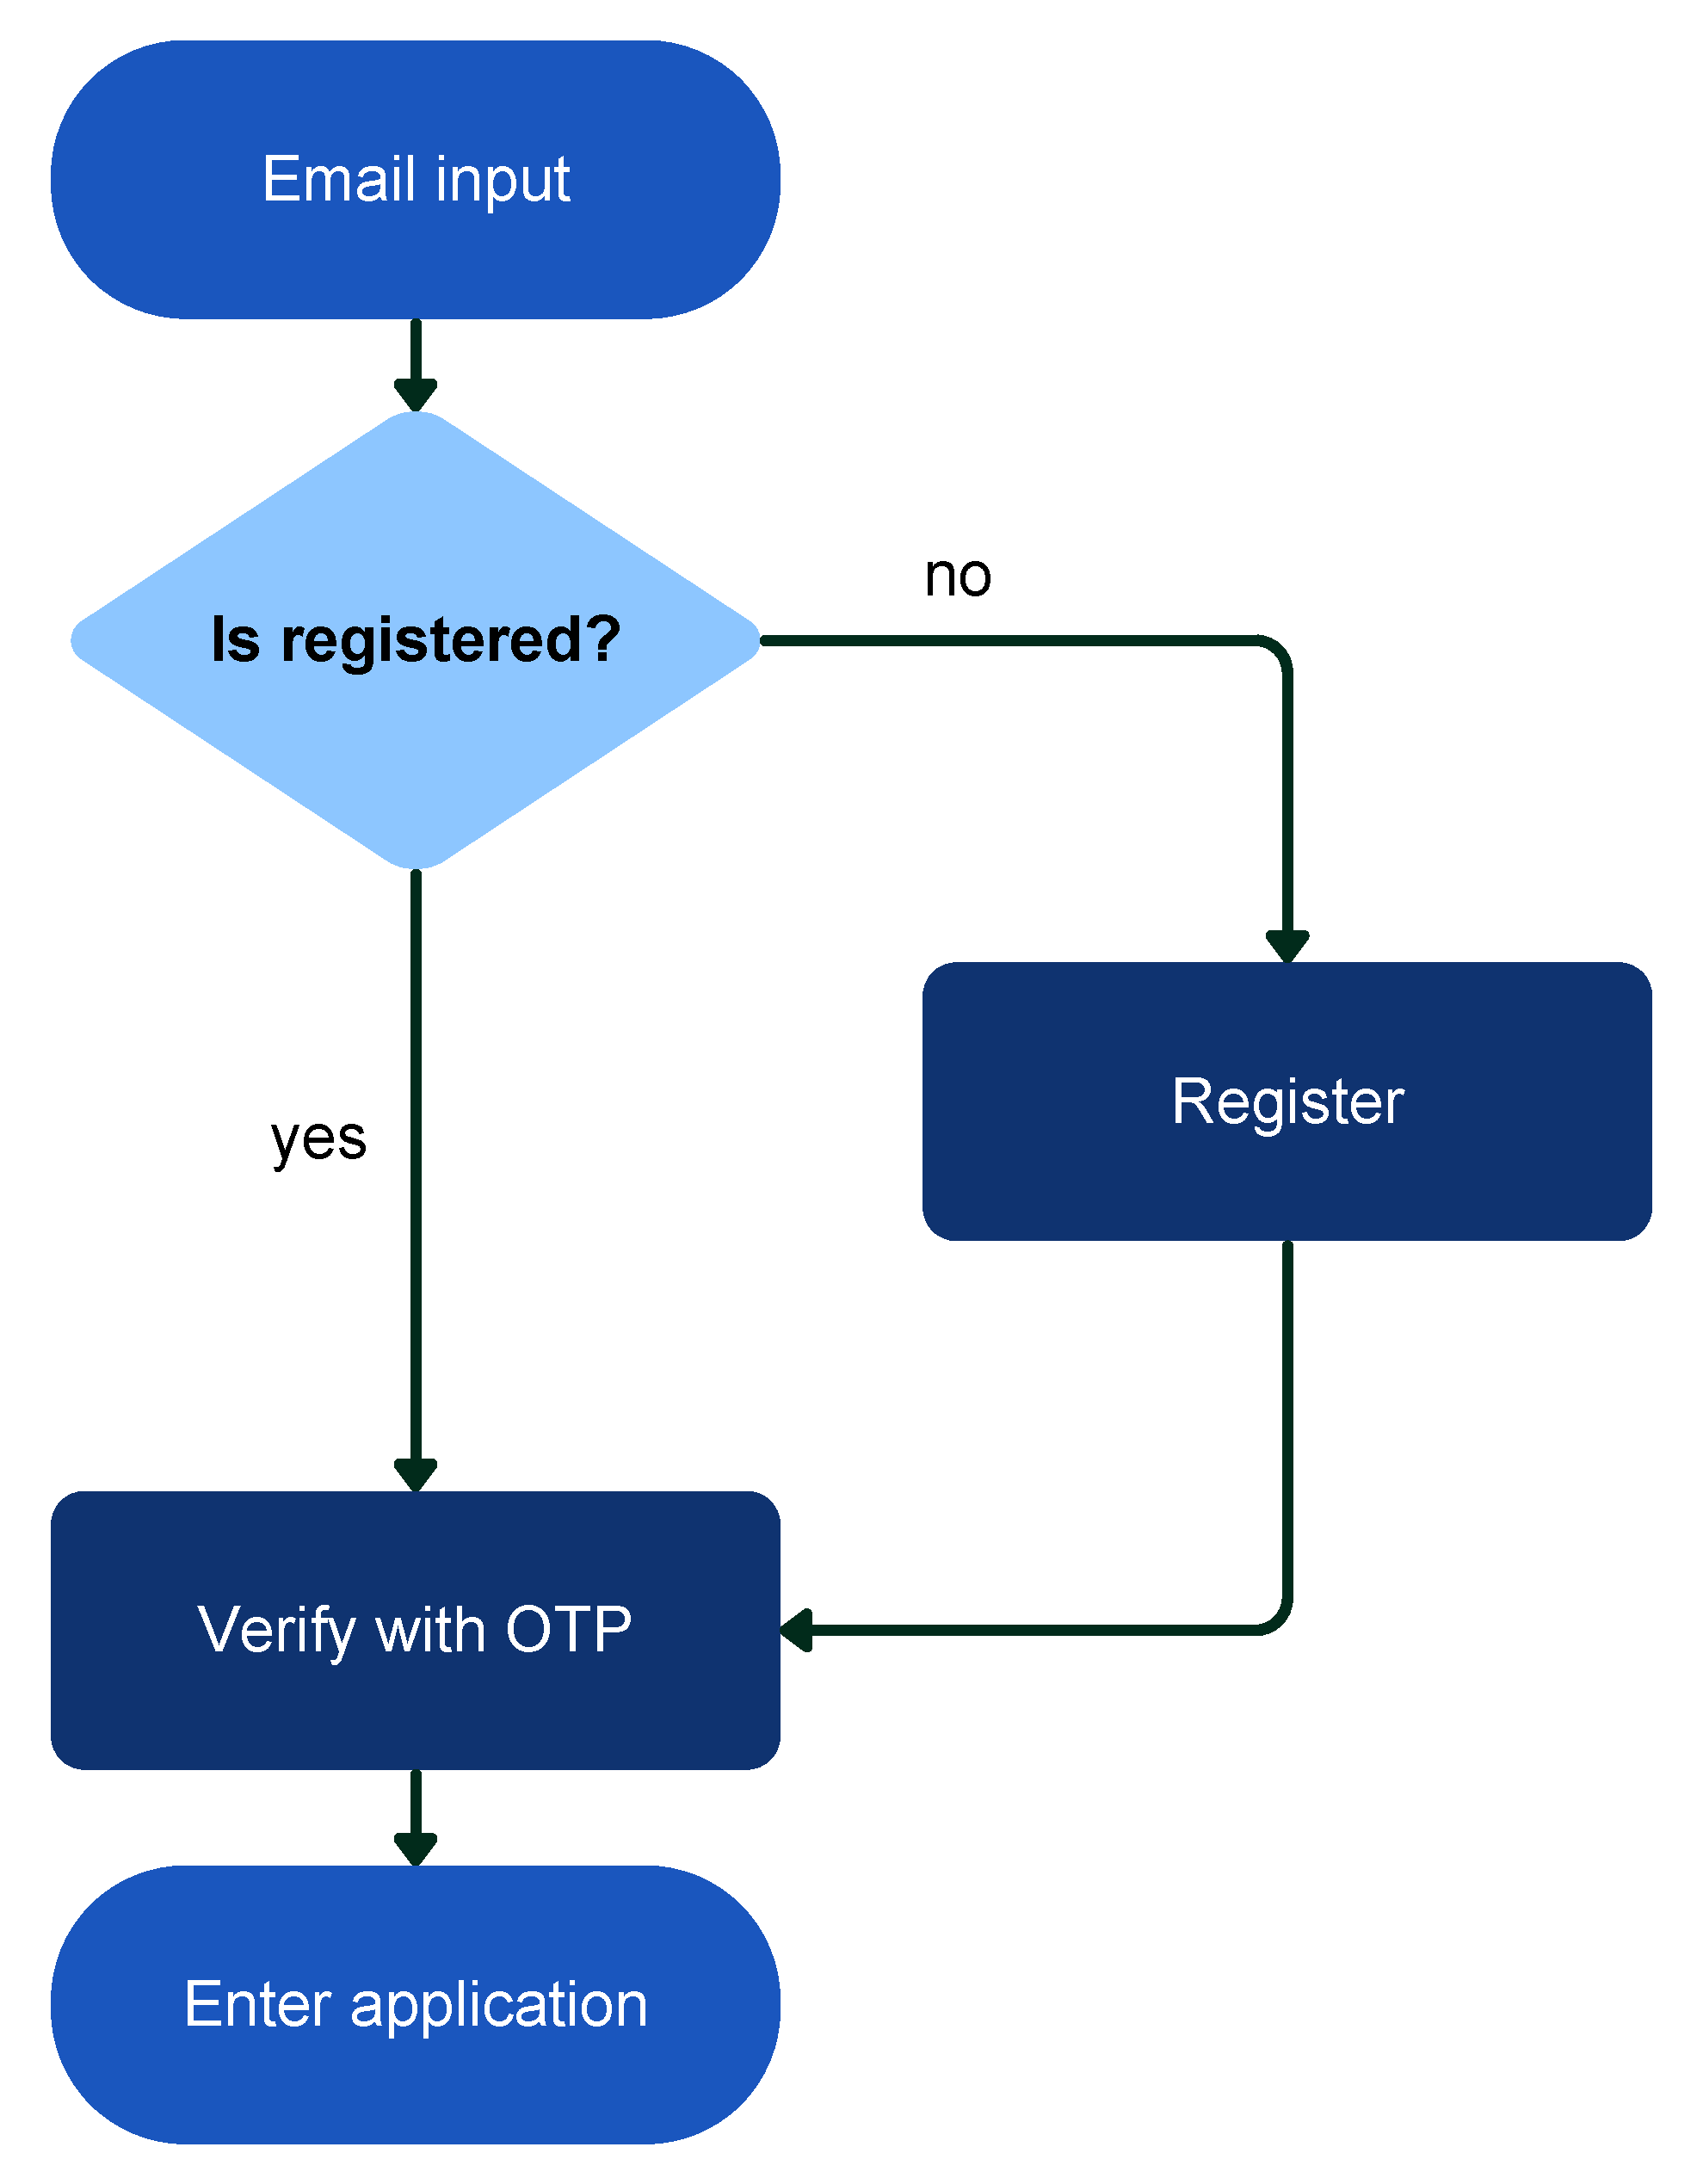
\includegraphics[width=0.5\textwidth]{obrazky-figures/implementacia-flow-diagram.pdf}
    \caption{Vývojový diagram toku autentifikácie v aplikácii Office Hours.
Diagram znázorňuje jednotlivé kroky procesu od spustenia aplikácie
cez zadanie e-mailovej adresy až po overenie jednorazovým OTP kódom
a udelenie prístupu k dátam systému.}
    \label{fig:flowdiagram}
\end{figure}

\section{Komunikácia s API a perzistencia dát}
\label{sec:impl-api}

\subsection{Trieda ApiService}

Všetka sieťová komunikácia aplikácie je sústredená v triede \textbf{ApiService}. Trieda je organizovaná do piatich logických sekcií: autentifikácia, používatelia, miestnosti, bloky a sloty. Každé volanie využíva balíček \textbf{http} a pristupuje k rovnakému základnému URL uloženému v triede \textbf{Constants}.

Spoločná pomocná metóda \textbf{\_headers()} zostavuje HTTP hlavičky pre každú požiadavku. Okrem \textbf{Content-Type: application/json} vkladá hlavičku \textbf{Authorization: Bea\-rer <token>} s aktuálnym JWT tokenom načítaným zo \textbf{SessionManager}. Tým je overenie identity zaistené pre každé chránené volanie bez toho, aby ho bolo potrebné riešiť na strane jednotlivých ViewModelov. Spracovanie neautorizovaných odpovedí je centralizované v metóde \textbf{\_checkUnauthorized()}, ktorá je volaná bezprostredne po každej HTTP odpovedi. Ak server vráti kód 401, metóda automaticky presmeruje používateľa na prihlasovaciu obrazovku. Ostatné chybové kódy sú riešené lokálne: nenaplnené podmienky úspechu vedú k vyhodeniu výnimky \textbf{Exception}, ktorú zachytí try-catch blok vo volajúcom ViewModeli. Výsledky úspešných volaní sú deserializované z JSON formátu a namapované na typované modelové triedy prostredníctvom metódy \textbf{fromJson}.

\subsection{Perzistencia dát a ukladanie relácie}
\label{subsec:impl-secure}
Aplikácia rozdeľuje perzistenciu dát do dvoch vrstiev podľa citlivosti informácií. Necitlivé údaje relácie – e-mailová adresa, rola, meno, dôvod návštevy, nastavenie témy a notifikácií – sú ukladané prostredníctvom triedy \textbf{UserPreferences}, ktorá obaľuje balíček \textbf{shared\_preferences}. Metóda \textbf{saveItem()} dynamicky zvolí správny setter (\textbf{setString}, \textbf{setBool} alebo \textbf{setInt}) podľa typu hodnoty, čo umožňuje jednotné rozhranie pre ukladanie rôznych dátových typov. JWT token je ukladaný oddelene v triede \textbf{SecureUserStorage} využívajúcej balíček \textbf{flutter\_secure\_storage} s Android Keystore, pričom je prístupný výlučne cez metódy \textbf{saveToken()}, \textbf{getToken()} a \textbf{removeToken()}.

Obe úložiská sú zastrešené triedou \textbf{SessionManager}, ktorá pri štarte aplikácie načíta celú reláciu do operačnej pamäte metódou \textbf{load()} a počas behu ju udržiava synchronizovanú s perzistentným úložiskom prostredníctvom individuálnych aktualizačných metód ako \textbf{updateFullName()} či \textbf{updateVisibility()}. Vďaka tomu ViewModely pristupujú k údajom relácie priamo z pamäte bez asynchrónnych čítaní z disku.

\subsection{Spracovanie chýb a validácia vstupov}

Validácia formulárových vstupov je sústredená v triede \textbf{Validator}. Metóda \textbf{validateEmail()} overuje prítomnosť znaku \textbf{@} a neprázdnych reťazcov na oboch stranách pomocou regulárneho výrazu a pri neúspešnej validácii zobrazí toast so zrozumiteľnou chybovou správou. Metóda \textbf{validateNotEmpty()} overuje neprázdnosť hodnoty a o zobrazenie správy sa stará volajúci kód.

Chyby vznikajúce pri sieťovej komunikácii sú zachytávané priamo vo ViewModeloch. Každé volanie \textbf{ApiService} je obalené blokom try-catch. Pri zachytení výnimky ViewModel resetuje príznak \textbf{isLoading} a prostredníctvom triedy \textbf{NotifyUserUtils} zobrazí toast pomocou balíčka \textbf{fluttertoast}. Trieda \textbf{NotifyUserUtils} poskytuje jednotné rozhranie \textbf{showToast()}, ktoré na základe parametra \textbf{isError} prepína farebnú schému správy – chybové hlásenia sú zobrazené s červeným pozadím, informatívne s neutrálnym.

\section{Implementácia konzultácií: miestnosti, bloky a sloty}
\label{sec:impl-konzultacie}
Táto sekcia opisuje implementáciu konzultačných miestností, blokov a slotov – od zobrazenia a rezervácie termínov až po ich vytváranie a úpravu.

\subsection{Hlavná obrazovka konzultácií a jej rozšírenie pre Majiteľa
}
\label{subsec:base-consultations}

Základom oboch hlavných pohľadov (Majiteľ aj Návštevník) je obrazovka \textbf{BaseConsultationsPage}. Ide o \textbf{StatefulWidget}, ktorý buď vytvorí vlastný \textbf{BaseConsultationsViewModel}, alebo preberie už existujúci ViewModel od volajúceho (typicky z \textbf{ConsultationsOwnerPage}). Po inicializácii obalí ViewModel pomocou \textbf{ChangeNotifierProvider.value} a vykreslí spoločné rozhranie: hornú lištu \textbf{AppBarMenu}, bočné menu \textbf{SliderMenu} a obsah, ktorý sa nachádza v triede \textbf{ConsultationsContent}.

V hornej časti obrazovky je umiestnený komponent \textbf{RoomSelectorButton}, ktorý je vložený do widgetu \textbf{StickyHeader}. Vďaka tomu zostáva výber miestnosti vizuálne prilepený k vrchu obrazovky pri skrolovaní zoznamu blokov. Pod ním nasleduje obsah konzultácií. Ak nie je vybratá žiadna miestnosť alebo používateľ nemá k dispozícii žiadnu miestnosť, zobrazuje sa komponent \textbf{NoRoomsFound} s prispôsobenou správou. Študent je nasmerovaný na \textbf{JoinRoomPage}, zatiaľ čo Majiteľ je vyzvaný na vytvorenie novej miestnosti cez \textbf{CreateRoomPage}.

\textbf{ConsultationsOwnerPage} poskytuje \textbf{BaseConsultationsPage} okrem ViewModelu aj množinu voliteľných widgetov a callbackov reprezentujúcich funkcie Majiteľa: tlačidlo \textbf{AddBlockButton} na vytváranie blokov, rozbaľovaciu ponuku \textbf{SettingsDropdownButton} na správu miestnosti (zobrazenie pripojených používateľov, úprava a zmazanie), tlačidlo \textbf{ShowHistoryButton} pre zobrazenie histórie slotov, tlačidlo \textbf{EditBlockButton} a dvojicu \textbf{AddSlotOnOutskirts} na pridanie slotu na začiatok alebo koniec bloku (obrázok~\ref{fig:owner-consultations}). Prepínač \textbf{AnimatedToggle} umožňuje Majiteľovi prepnúť sa do
návštevníckeho pohľadu. V tomto režime odovzdáva \textbf{ConsultationsOwnerPage}
všetky tieto parametre ako \textbf{null}, čím \textbf{BaseConsultationsPage}
vykreslí rozhranie bez administrátorských akcií.

\begin{figure}[t]
    \centering
    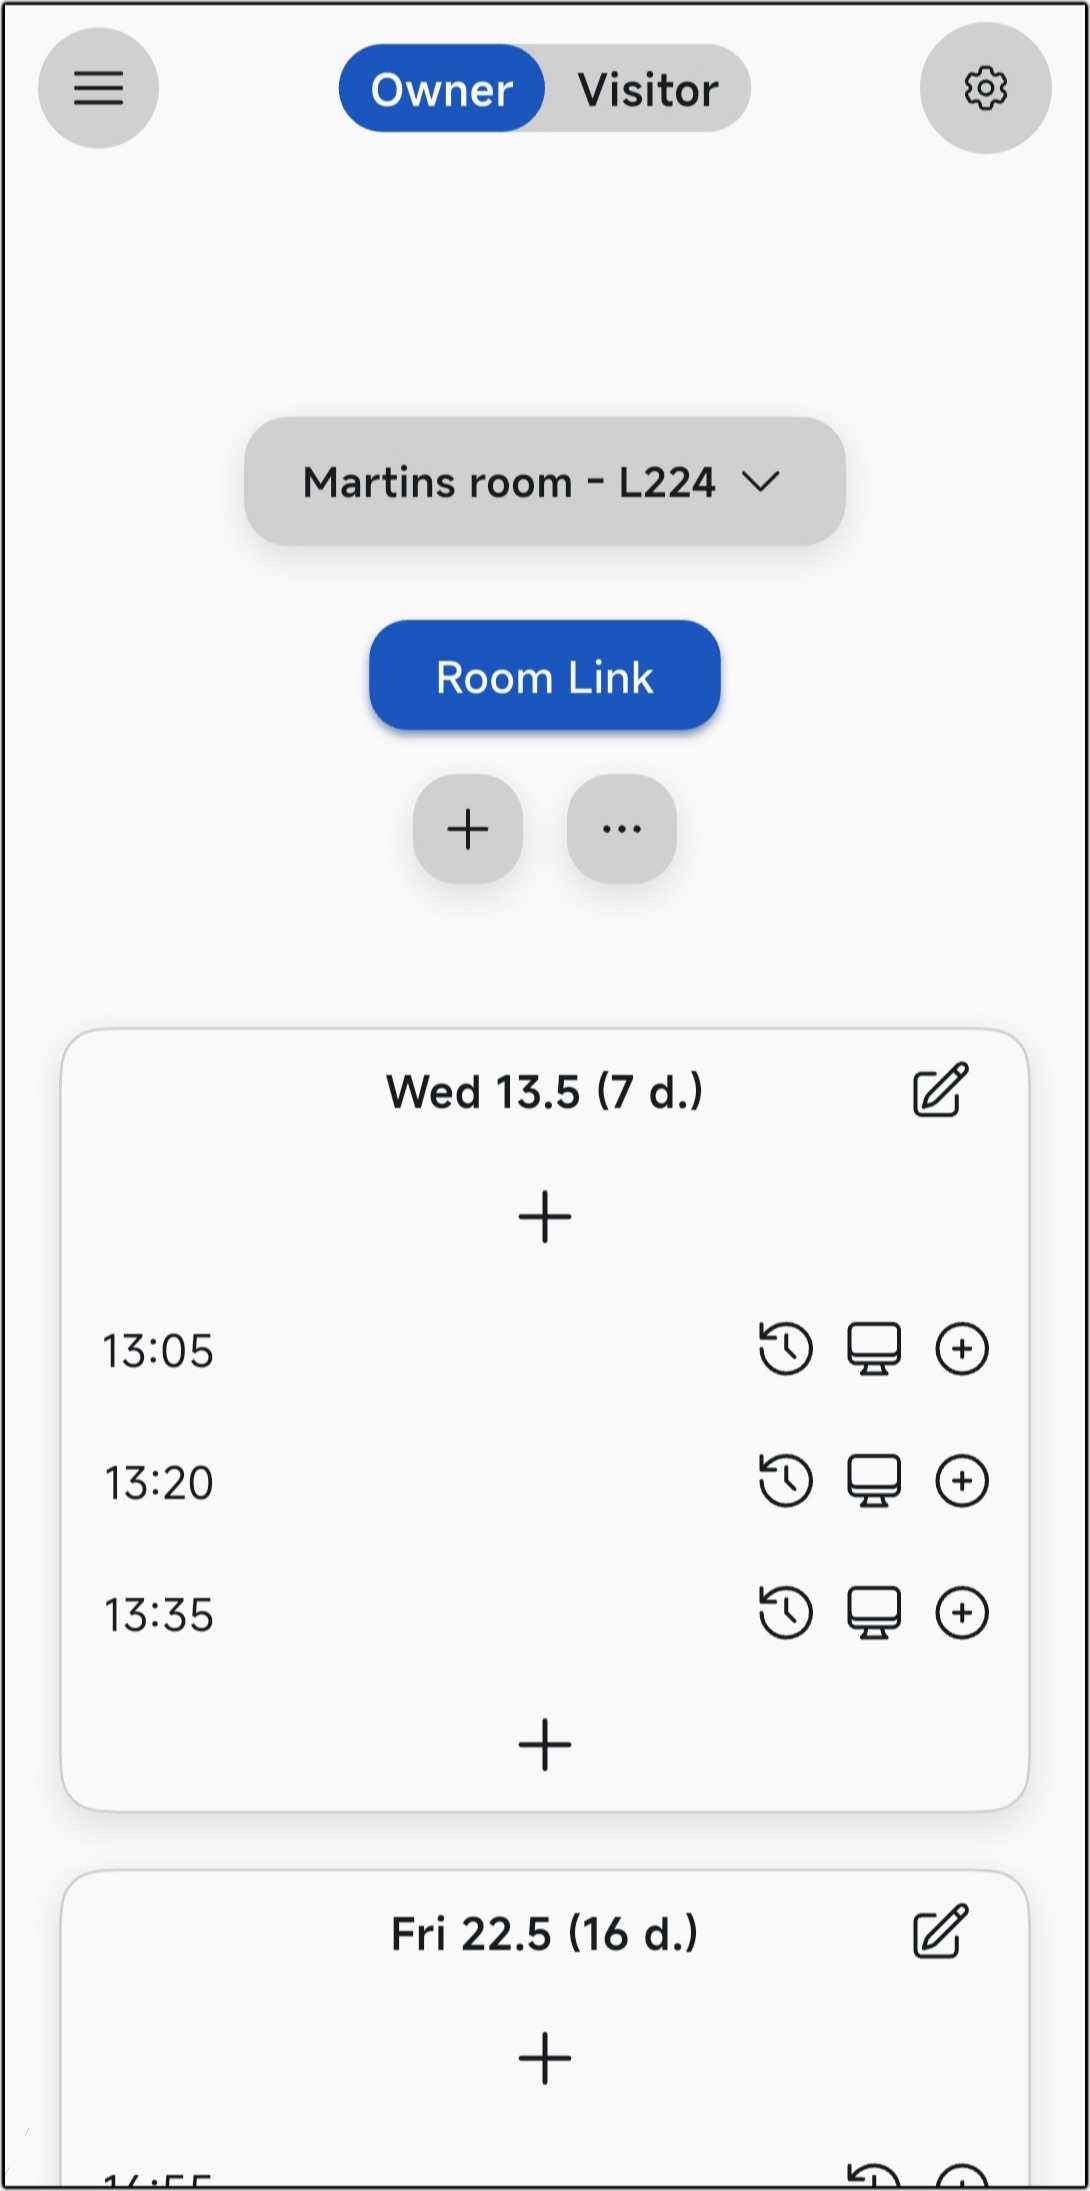
\includegraphics[width=0.4\textwidth]{obrazky-figures/implementacia-owner-example-app.png}
    \caption{Hlavná obrazovka konzultácií v pohľade Majiteľa. 
    V hornej lište je viditeľný prepínač \textit{Owner/Visitor} 
    implementovaný ako \textbf{AnimatedToggle}. Pod ním je prilepený 
    \textbf{RoomSelectorButton} s názvom aktuálne vybranej miestnosti. 
    Tlačidlá \uv{+} a \uv{...} slúžia na vytvorenie nového bloku 
    a správu miestnosti. Každý blok zobrazuje dátum s relatívnym 
    označením počtu dní a ikonu úpravy vpravo hore. 
    Sloty vo vnútri bloku obsahujú čas za\-čiatku a akčné ikony 
    pre históriu, typ konzultácie a pridanie slotu.}
    \label{fig:owner-consultations}
\end{figure}

\subsection{Zobrazenie blokov a slotov, rezervácia a zrušenie slotu}
\label{subsec:bloky-sloty}

Samotný zoznam blokov v aktuálne vybranej miestnosti je implementovaný v triede \textbf{ConsultationsContent}. Táto trieda najprv vykreslí tlačidlo \textbf{Room Link}, ktoré otvára externý odkaz priradený k miestnosti a voliteľný riadok s tlačidlami pre Majiteľa (vytvoriť blok, nastavenia miestnosti). Nasleduje buď text \uv{No upcoming consultations found.}, ak miestnosť neobsahuje žiadne bloky, alebo zoznam blokov zoradených chronologicky podľa dátumu. Každý blok je reprezentovaný kartou \textbf{ConsultationBlockCard}.

\textbf{ConsultationBlockCard} zobrazuje hlavičku s dátumom bloku a akciou v pravom hornom rohu. V študentskom pohľade je to ikona zvončeka, ktorá umožňuje prihlásenie alebo odhlásenie z e-mailových notifikácií pre daný blok. V pohľade Majiteľa je táto ikona nahradená tlačidlom na úpravu bloku cez \textbf{editBlockButton}. Pod hlavičkou sa nachádza voliteľné tlačidlo na vloženie slotu na začiatok zoznamu (iba pre Majiteľa), zoznam slotov a tlačidlo na pridanie slotu na koniec bloku. Tlačidlo na pridanie slotu má ikonku \uv{plus} a počas odosielania požiadavky na rezerváciu sa mení na animovaný indikátor. Zoznam slotov je vykreslený pomocou \textbf{ListView.builder}. Každý slot je zabalený v \textbf{Selector}, ktorý sleduje dvojicu hodnôt \textbf{isTakingSlot} a \textbf{isOptimisticallyReleased}. Tým sa zabezpečí, že pri rezervácii alebo uvoľnení slotu sa prekreslí iba daný slot, nie celý zoznam.

O samotné vykreslenie slotu sa stará widget \textbf{SlotWidget}. Na základe dát
z \textbf{SlotModel} a stavu vo ViewModeli najprv určí, či je slot voľný
(\textbf{takenBy == null} alebo prebieha optimistické uvoľnenie), rezervovaný
prihláseným používateľom, alebo rezervovaný iným študentom. Podľa toho zvolí
jeden z troch špecializovaných widgetov: \textbf{CurrentUserSlot},
\textbf{FreeSlot} alebo \textbf{AnotherUsersSlot} – ich vizuálne rozlíšenie
je popísané v kapitole~\ref{chap:navrh}. Widget \textbf{CurrentUserSlot}
navyše obsahuje tlačidlo na uvoľnenie, ktoré pri zrušení rezervácie v krátkom
časovom predstihu zobrazí varovný dialóg.

\textbf{SlotWidget} zároveň vlastní dve spodné karty (bottom sheets).
Pri ťuknutí na voľný slot otvorí \textbf{TakeSlotBottomSheet} s obsahom
navrhnutým v kapitole~\ref{chap:navrh}. Po potvrdení zavolá callback
\textbf{onTakeSlot()} s poznámkou a príznakom online a okamžite kartu zavrie.
Pri kliknutí na obsadený slot môže byť zobrazená \textbf{TypeBottomSheet},
ktorá umožňuje Majiteľovi zmeniť typ konzultácie bez rušenia rezervácie
a návštevníkovi zmeniť typ jeho vlastnej konzultácie.

\begin{figure}[t]
    \centering
    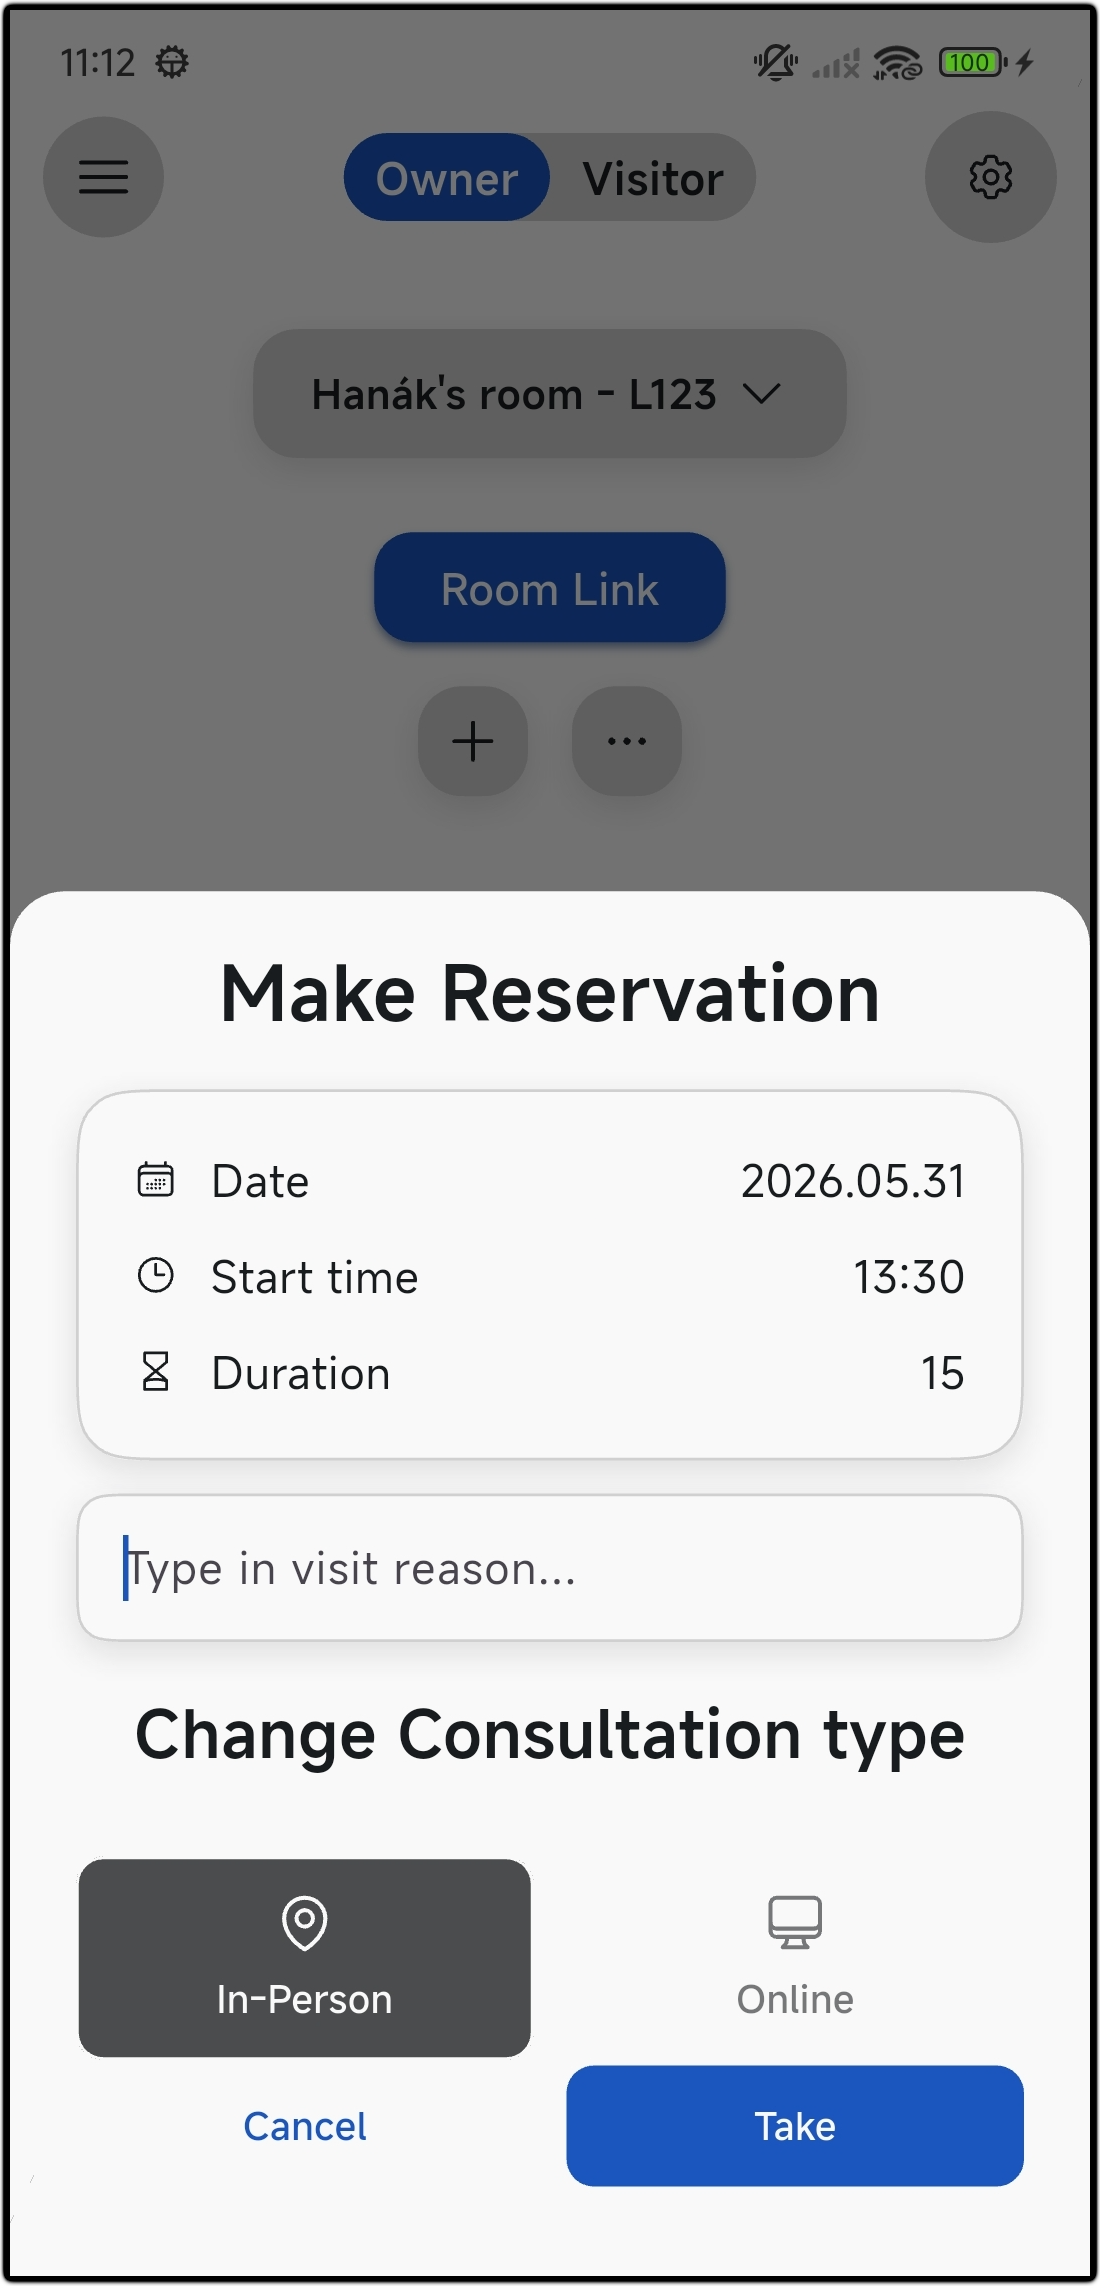
\includegraphics[width=0.4\textwidth]{obrazky-figures/implementacia-slot-take-dialog.png}
    \caption{Spodná karta \textbf{TakeSlotBottomSheet} zobrazená po kliknutí
    na voľný slot. Obsahuje prehľad vybraného termínu (dátum, čas, trvanie),
    textové pole pre zadanie dôvodu návštevy a prepínač typu konzultácie
    (\textit{In-Person}/\textit{Online}). Tlačidlo \uv{Take} potvrdí rezerváciu
    a kartu okamžite zavrie.}
    \label{fig:take-slot-dialog}
\end{figure}

\begin{figure}[t]
    \centering
    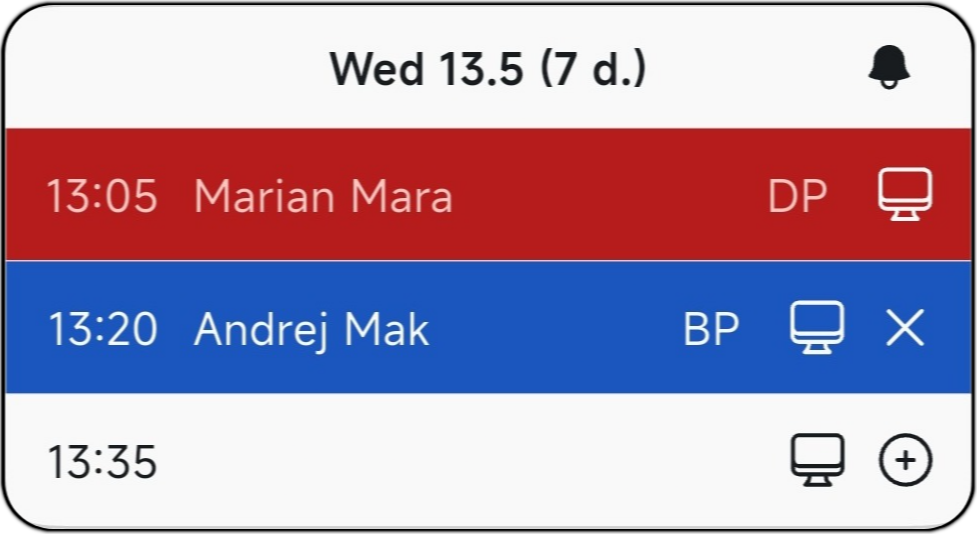
\includegraphics[width=0.4\textwidth]{obrazky-figures/implementacia-slot-states-example.png}
    \caption{Tri vizuálne stavy widgetu \textbf{SlotWidget} v rámci 
    jedného bloku. Červený slot predstavuje variant 
    \textbf{AnotherUsersSlot} – termín rezervovaný iným študentom. 
    Modrý slot zodpovedá variantu \textbf{CurrentUserSlot} – 
    termín prihláseného používateľa s tlačidlom na zrušenie rezervácie. 
    Biely slot je voľný termín (\textbf{FreeSlot}) 
    s ikonou na pridanie slotu za neho. Skratky pri slotoch 
    označujú dôvod návštevy študenta.}
    \label{fig:slot_states_example}
\end{figure}

\subsection{Pripojenie do miestnosti (JoinRoomPage)}
\label{subsec:join-room}

Obrazovka \textbf{JoinRoomPage} umožňuje študentom vyhľadať a pripojiť sa k ľubovoľnej dostupnej miestnosti. Po inicializácii ViewModel načíta zoznam všetkých miestností, ktoré sú študentovi dostupné podľa nastavených e-mailových domén a adries. Horná časť obrazovky obsahuje formulár s komponentom \textbf{Autocomplete}, ktorý nad zoznamom miestností ponúka dynamické dopĺňanie podľa zadaného textu. Zoznam možností sa filtruje podľa podreťazca v názve miestnosti a miestnosti, do ktorých je študent už prihlásený, sú z ponuky automaticky skryté. 

Okrem výberu zo zoznamu \textbf{Autocomplete} priebežne kontroluje aj manuálne zadanie názvu – ak používateľ zadá presný názov existujúcej miestnosti bez toho, aby položku vybral zo zoznamu, ViewModel vyhodnotí zhodu a nastaví vybranú miestnosť. Po stlačení tlačidla \uv{Join room} sa študent pokúsi do zvolenej miestnosti pripojiť. V spodnej časti stránky je zoznam miestností, do ktorých je študent už pripojený.

\subsection{Vytvorenie a editácia bloku}
\label{subsubsec:block-create-edit}

Vytváranie nových blokov je realizované na obrazovke \textbf{CreateBlock}.
Formulár pokrýva parametre bloku definované v návrhu
(kapitola~\ref{chap:navrh}). Výber dátumov zabezpečuje dialóg
\textbf{CustomDateRangePickerDialog}, ktorý podporuje výber jedného dňa,
rozsahu alebo viacerých nesúvislých dní podľa aktuálne zvoleného režimu.
Zvolený rozsah je zobrazený v textovej podobe priamo v hlavnom formulári
a pri potvrdení je uložený do ViewModelu.

Časová konfigurácia je riešená pomocou komponentu \textbf{CustomTimeDurationPicker}.
Po zadaní počtu slotov ViewModel vypočíta koncový čas bloku a zobrazí ho
v neklikateľnom poli \textbf{End Time} (obrázok~\ref{fig:create-block}).
Tlačidlo „Create" po stlačení zavolá metódu \textbf{createBlock(roomId, onSuccess)},
ktorá po úspešnom vytvorení bloku spustí callback \textbf{onSuccess} -
typicky \textbf{viewModel.loadRoom()} na \textbf{ConsultationsOwnerPage} -
a tým obnoví zoznam blokov v pôvodnej obrazovke.

Úprava existujúceho bloku prebieha na obrazovke \textbf{EditBlockPage}. Po načítaní bloku ViewModel zobrazí názov miestnosti, dátum bloku a zoznam slotov v komponentoch \textbf{SlotRow}. Každý riadok obsahuje čas slotu, poznámku o obsadenosti, ikonku online/offline a tlačidlo na zmazanie. Okrem toho obrazovka ponúka funkciu \textbf{copyBlock}, ktorá umožňuje skopírovať celý blok vrátane rozloženia slotov na iné dátumy opäť pomocou dialógu \textbf{CustomDateRangePickerDialog}. Prepínač \uv{Online} na úrovni bloku umožňuje hromadne prepnúť typ všetkých slotov (napríklad na online z dôvodu choroby), pričom po úspešnom uložení sa opäť volá callback \textbf{onSuccess} pre obnovu rodičovskej obrazovky (obrázok~\ref{fig:edit-block}).
\begin{figure}[t]
    \centering
    \begin{minipage}[t]{0.48\textwidth}
        \centering
        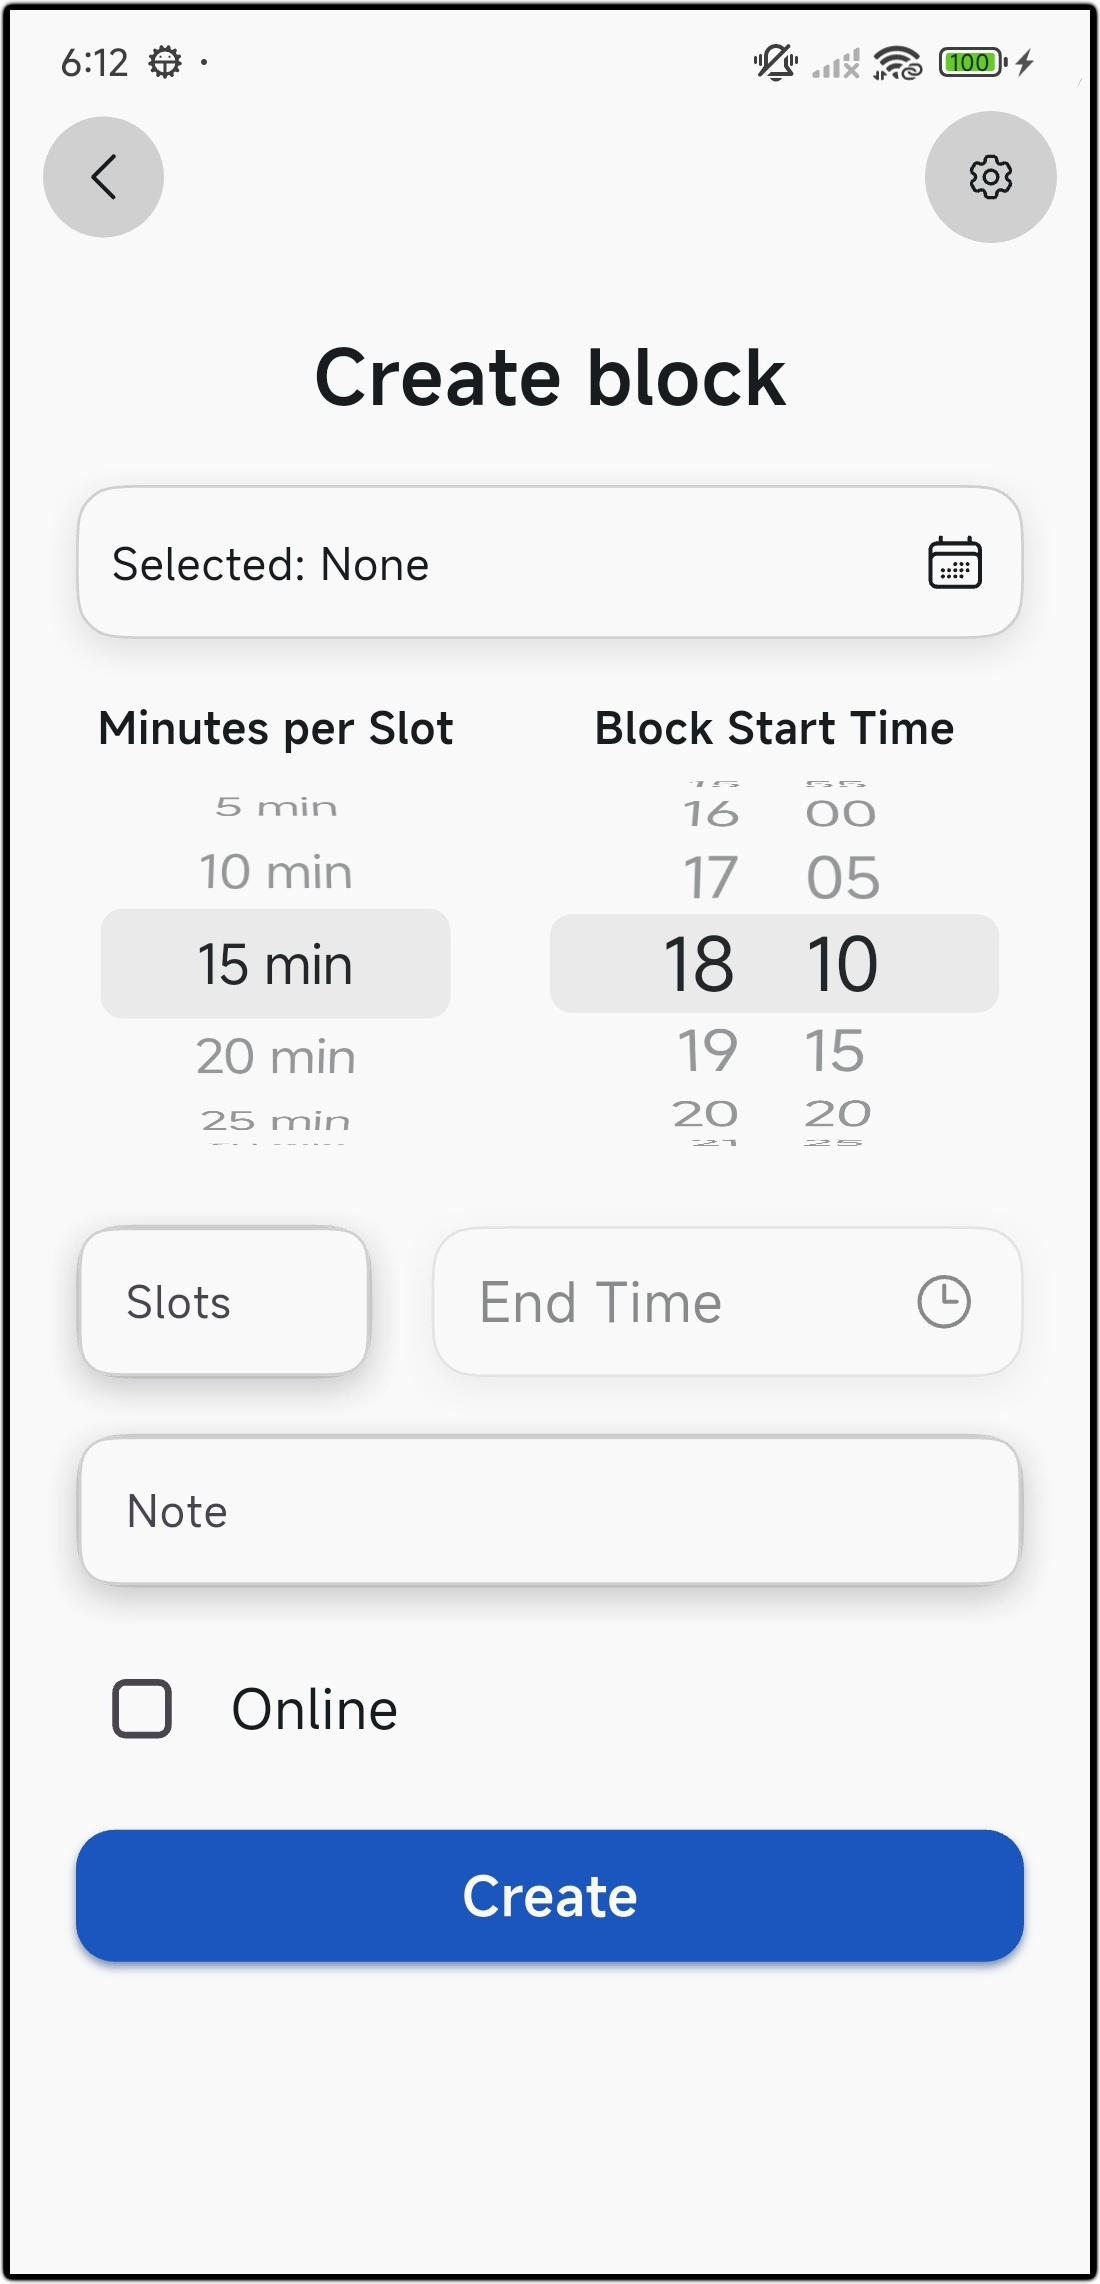
\includegraphics[width=\textwidth]{obrazky-figures/implementacia-create-block.png}
        \caption{Obrazovka \textbf{CreateBlock} s formulárom pre výber dátumu,
        počtu slotov a trvania pomocou \textbf{CustomTimeDurationPicker}.}
        \label{fig:create-block}
    \end{minipage}
    \hfill
    \begin{minipage}[t]{0.48\textwidth}
         \centering
        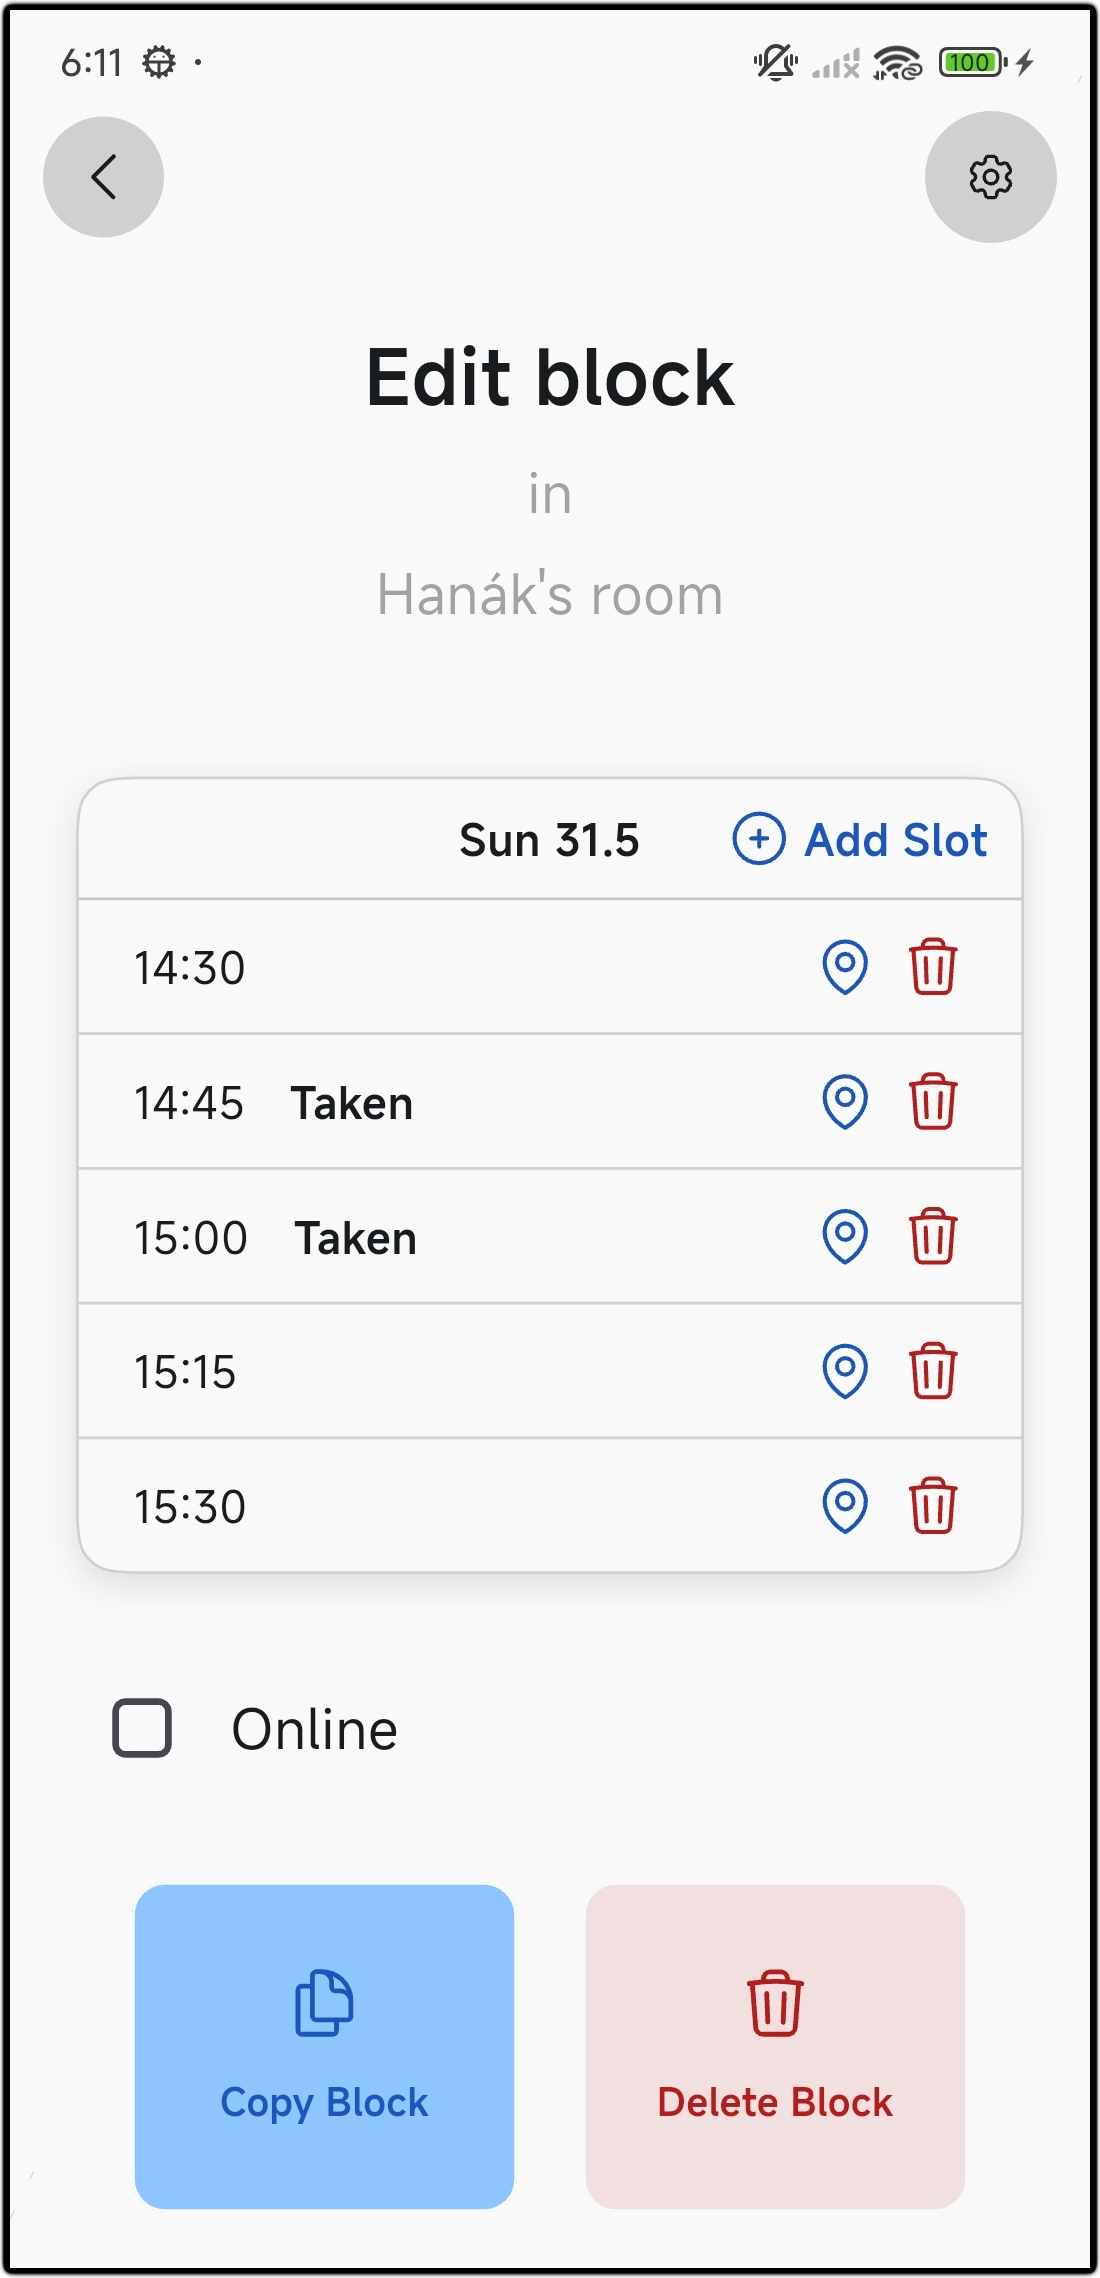
\includegraphics[width=\textwidth]{obrazky-figures/implementacia-edit-block.png}
        \caption{Obrazovka \textbf{EditBlockPage} so zoznamom slotov, prepínačom hromadnej zmeny
        typu konzultácie na úrovni bloku a možnosťami kopírovať a vymazať blok.}
        \label{fig:edit-block}
    \end{minipage}
\end{figure}

\subsection{Vytvorenie a editácia miestnosti}
\label{subsubsec:room-create-edit}

Vytváranie miestnosti je realizované obrazovkou \textbf{CreateRoomPage},
ktorá je implementovaná ako \textbf{StatelessWidget}. Využíva spoločný
komponent \textbf{RoomFormBody} pokrývajúci všetky atribúty miestnosti, definované v návrhu (kapitola~\ref{chap:navrh}). Po stlačení tlačidla
„Create" sa zavolá metóda \textbf{createRoom()}, ktorá vstupy odošle na server (obrázok~\ref{fig:create-room}).

\textbf{EditRoomPage} zdieľa rovnaký formulár \textbf{RoomFormBody}, avšak ako \textbf{StatefulWidget} v metóde \textbf{initState()} najprv načíta existujúce dáta miestnosti z API a predvyplní nimi príslušné textové polia a zoznam \textbf{acceptedEmails}.

\begin{figure}[t]
    \centering
    \begin{minipage}[t]{0.45\textwidth}
        \centering
        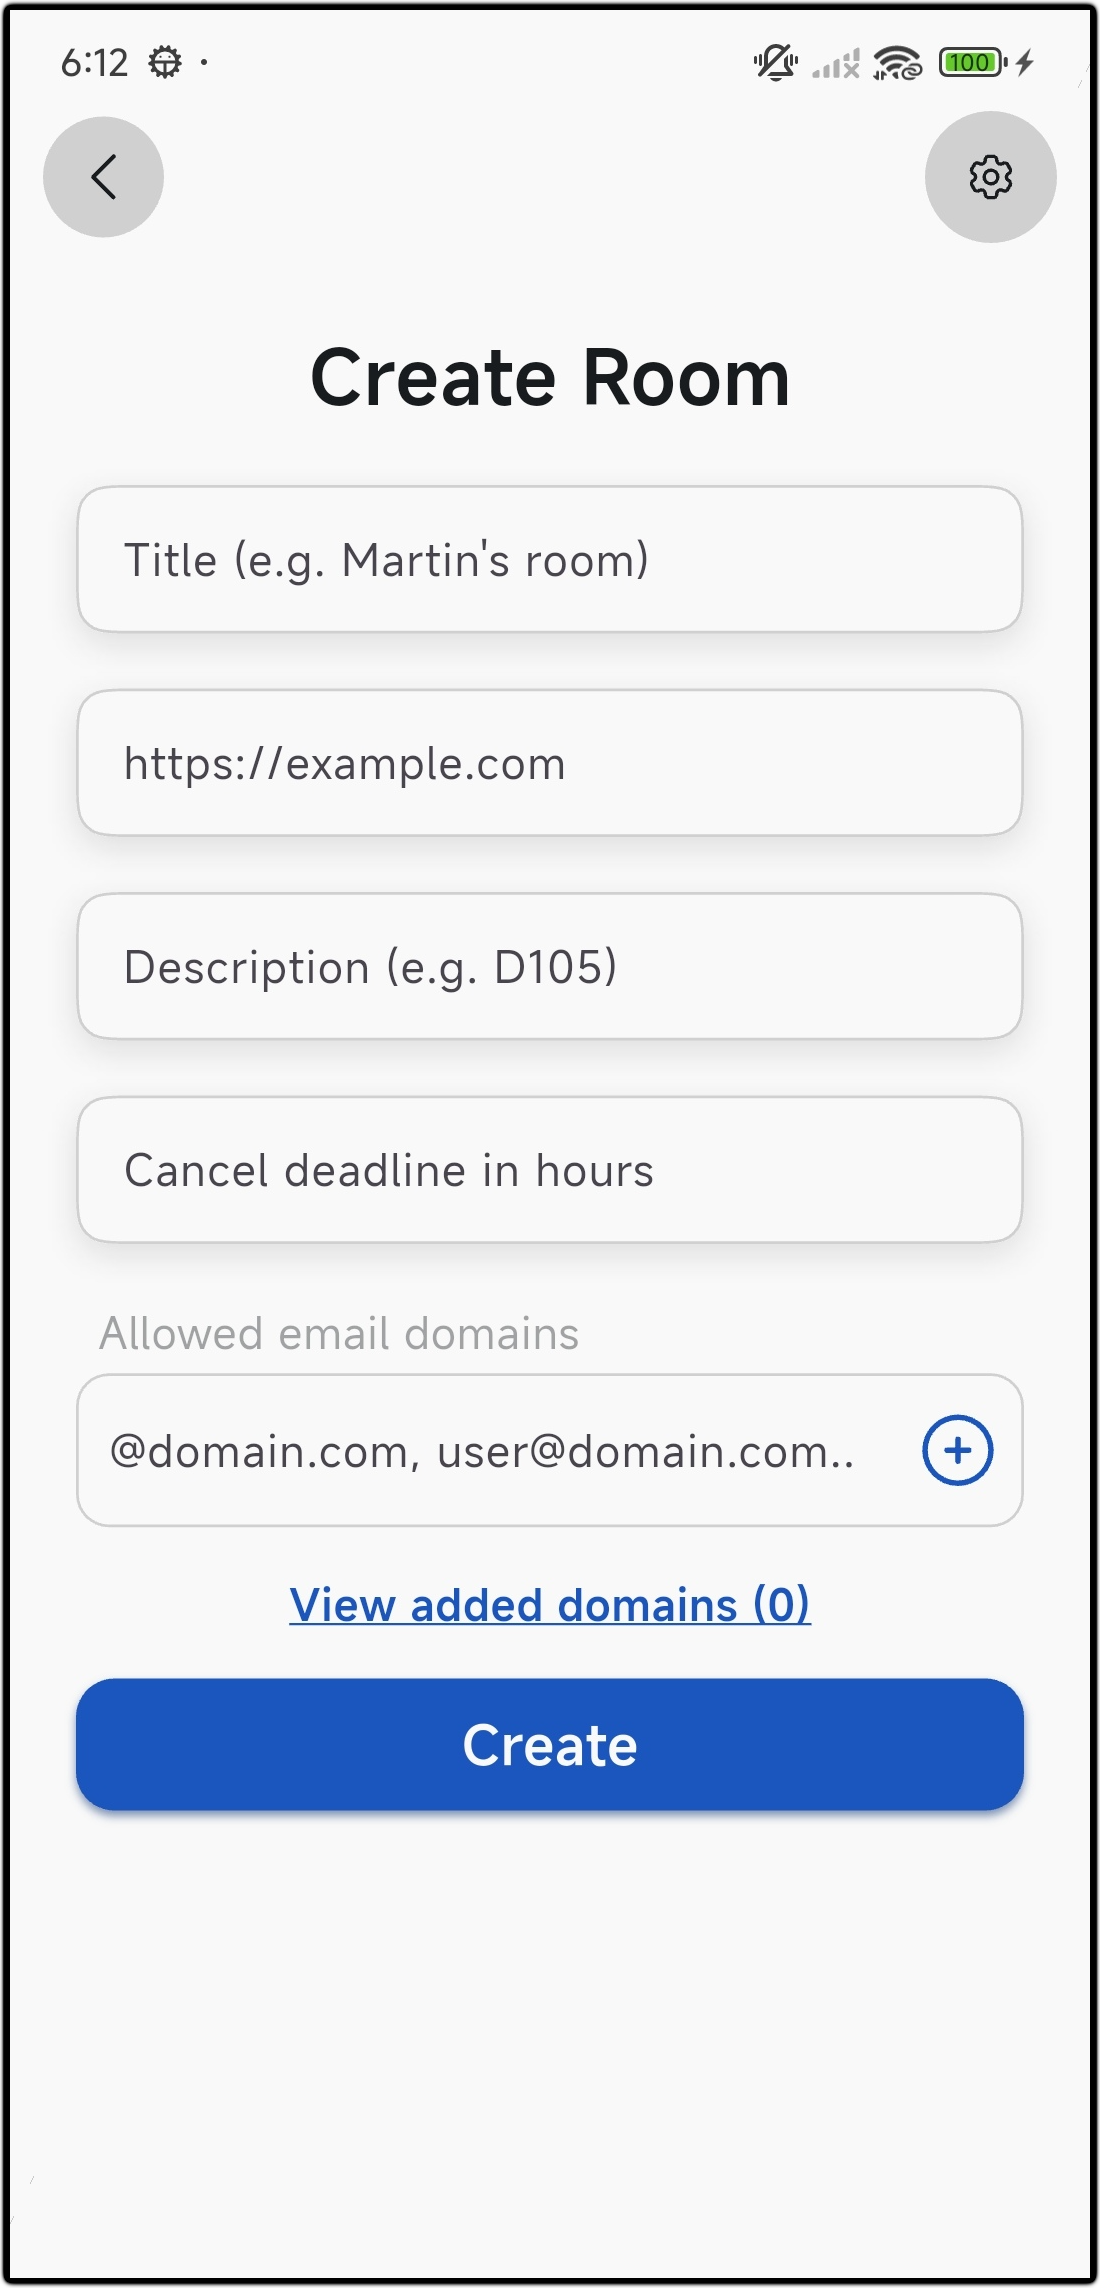
\includegraphics[width=\textwidth]{obrazky-figures/implementacia-create-room.png}
        \caption{Obrazovka \textbf{CreateRoomPage} s formulárom
        \textbf{RoomFormBody} pre zadanie názvu, popisu, externého
        odkazu a zoznamu povolených e-mailových domén.}
        \label{fig:create-room}
    \end{minipage}
    \hfill
    \begin{minipage}[t]{0.45\textwidth}
        \centering
        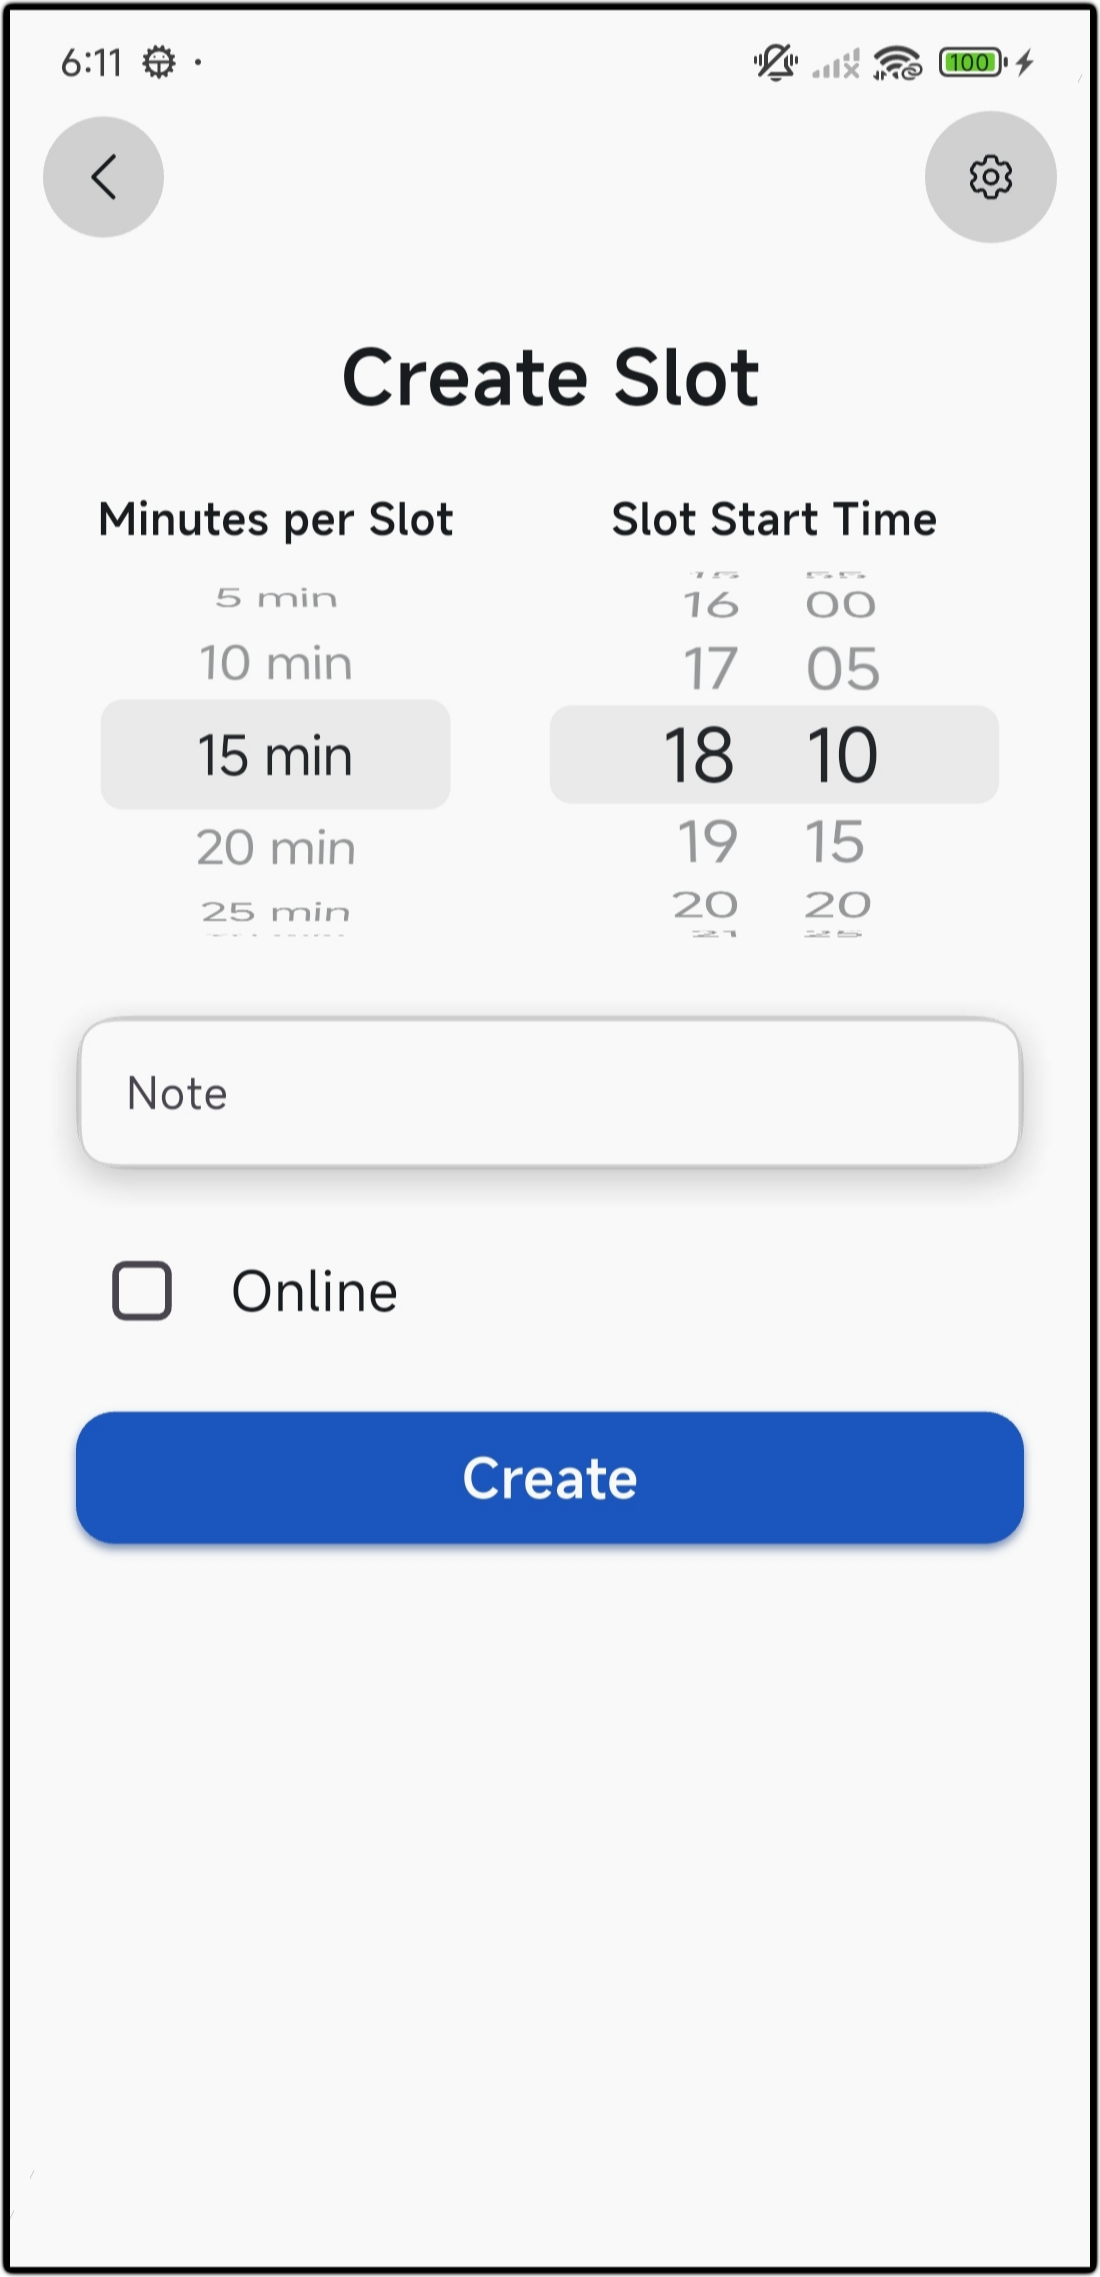
\includegraphics[width=\textwidth]{obrazky-figures/implementacia-create-slot.png}
        \caption{Obrazovka \textbf{AddSlotPage} s komponentom
        \textbf{CustomTimeDurationPicker} pre výber času začiatku
        a trvania nového slotu.}
        \label{fig:create-slot}
    \end{minipage}
\end{figure}

\subsection{Prehľad používateľov a história slotu}
\label{subsubsec:users-history}

Z pohľadu Majiteľa sú k dispozícii dve doplnkové obrazovky poskytujúce detailnejší prehľad o používaní miestnosti. \textbf{DisplayUsersInRoomPage} zobrazuje zoznam všetkých používateľov, ktorí sa pripojili do danej miestnosti. Obrazovka po načítaní dát zobrazí informáciu o prázdnom zozname, alebo zoznam e-mailových adries v tvare kariet. V hornej časti sa zároveň zobrazuje počet členov miestnosti.

História konkrétneho slotu je prístupná z pohľadu Majiteľa cez tlačidlo \textbf{ShowHistoryButton} na každom slote. Po stlačení sa otvorí \textbf{DisplaySlotHistoryPage}, ktorá vizuálne reprezentuje chronologický zoznam všetkých rezervácií daného slotu, vrátane informácie, kto a kedy slot obsadil alebo uvoľnil. Týmto spôsobom má Majiteľ k dispozícii možnosť spätne overiť históriu rezervácií daného slotu.

\subsection{Prehľad vlastných rezervácií}
\label{subsec:my-reservations}

Obrazovka \textbf{MyReservationsPage} bola pridaná na základe spätnej väzby
testerov, ktorí postrádali centrálny prehľad vlastných rezervácií naprieč
všetkými miestnosťami. Obrazovka je prístupná z hamburger menu a zobrazuje
všetky aktívne rezervácie prihláseného používateľa bez ohľadu na to,
do ktorej miestnosti patria.

Obrazovka je implementovaná ako \textbf{StatelessWidget}, ktorý pri zostrojení
vytvorí inštanciu \textbf{MyReservationsViewModel} a okamžite spustí
inicializáciu kaskádovým volaním \textbf{MyReservationsViewModel()..initialize()}.
Metóda \textbf{initialize()} vykoná dve sieťové volania:
\textbf{api.getMyReservations()} na získanie rezervovaných slotov
a \textbf{api.getAllRooms()} na získanie zoznamu miestností,
ktoré sú uložené v premennej \textbf{\_cachedRooms}.
Pomocná metóda \textbf{slotEssentials(index)} pre každý slot vráti mapu zobraziteľných hodnôt: názov miestnosti,
dátum, čas začiatku, trvanie, poznámku a príznaky prebiehajúcich operácií.
Kým prebieha načítavanie, zobrazuje sa indikátor.
Po jeho dokončení sa vykreslí zoznam kariet, alebo prázdny stav
\textbf{\_EmptyState} s výzvou na rezervovanie prvého termínu.

Každá karta umožňuje dve akcie. Klepnutím na ikonu krížika používateľ
zruší rezerváciu – metóda \textbf{releaseSlot()} slot okamžite odstráni
z lokálneho zoznamu a skutočné volanie API prebehne až následne.
Klepnutím na ikonu obrazovky alebo polohy sa otvorí
\textbf{ConsultationTypeBottomSheet}, kde používateľ potvrdí zmenu
typu konzultácie – metóda \textbf{changeType()} analogicky prehodí
príznak \textbf{is\_online} v lokálnej kópii ešte pred odpoveďou servera.
V prípade zlyhania ktorejkoľvek operácie sa stav obnoví z vopred
uloženého snapshotu a používateľovi sa zobrazí chybový toast.
Keďže obe akcie môžu prebiehať súčasne na rôznych kartách,
ViewModel sleduje ich stav v mapách \textbf{\_optimisticallyReleased}
a \textbf{\_changingType} s kľúčom podľa identifikátora slotu.


\begin{figure}[t]
    \centering
    \begin{minipage}[t]{0.45\textwidth}
       \centering
    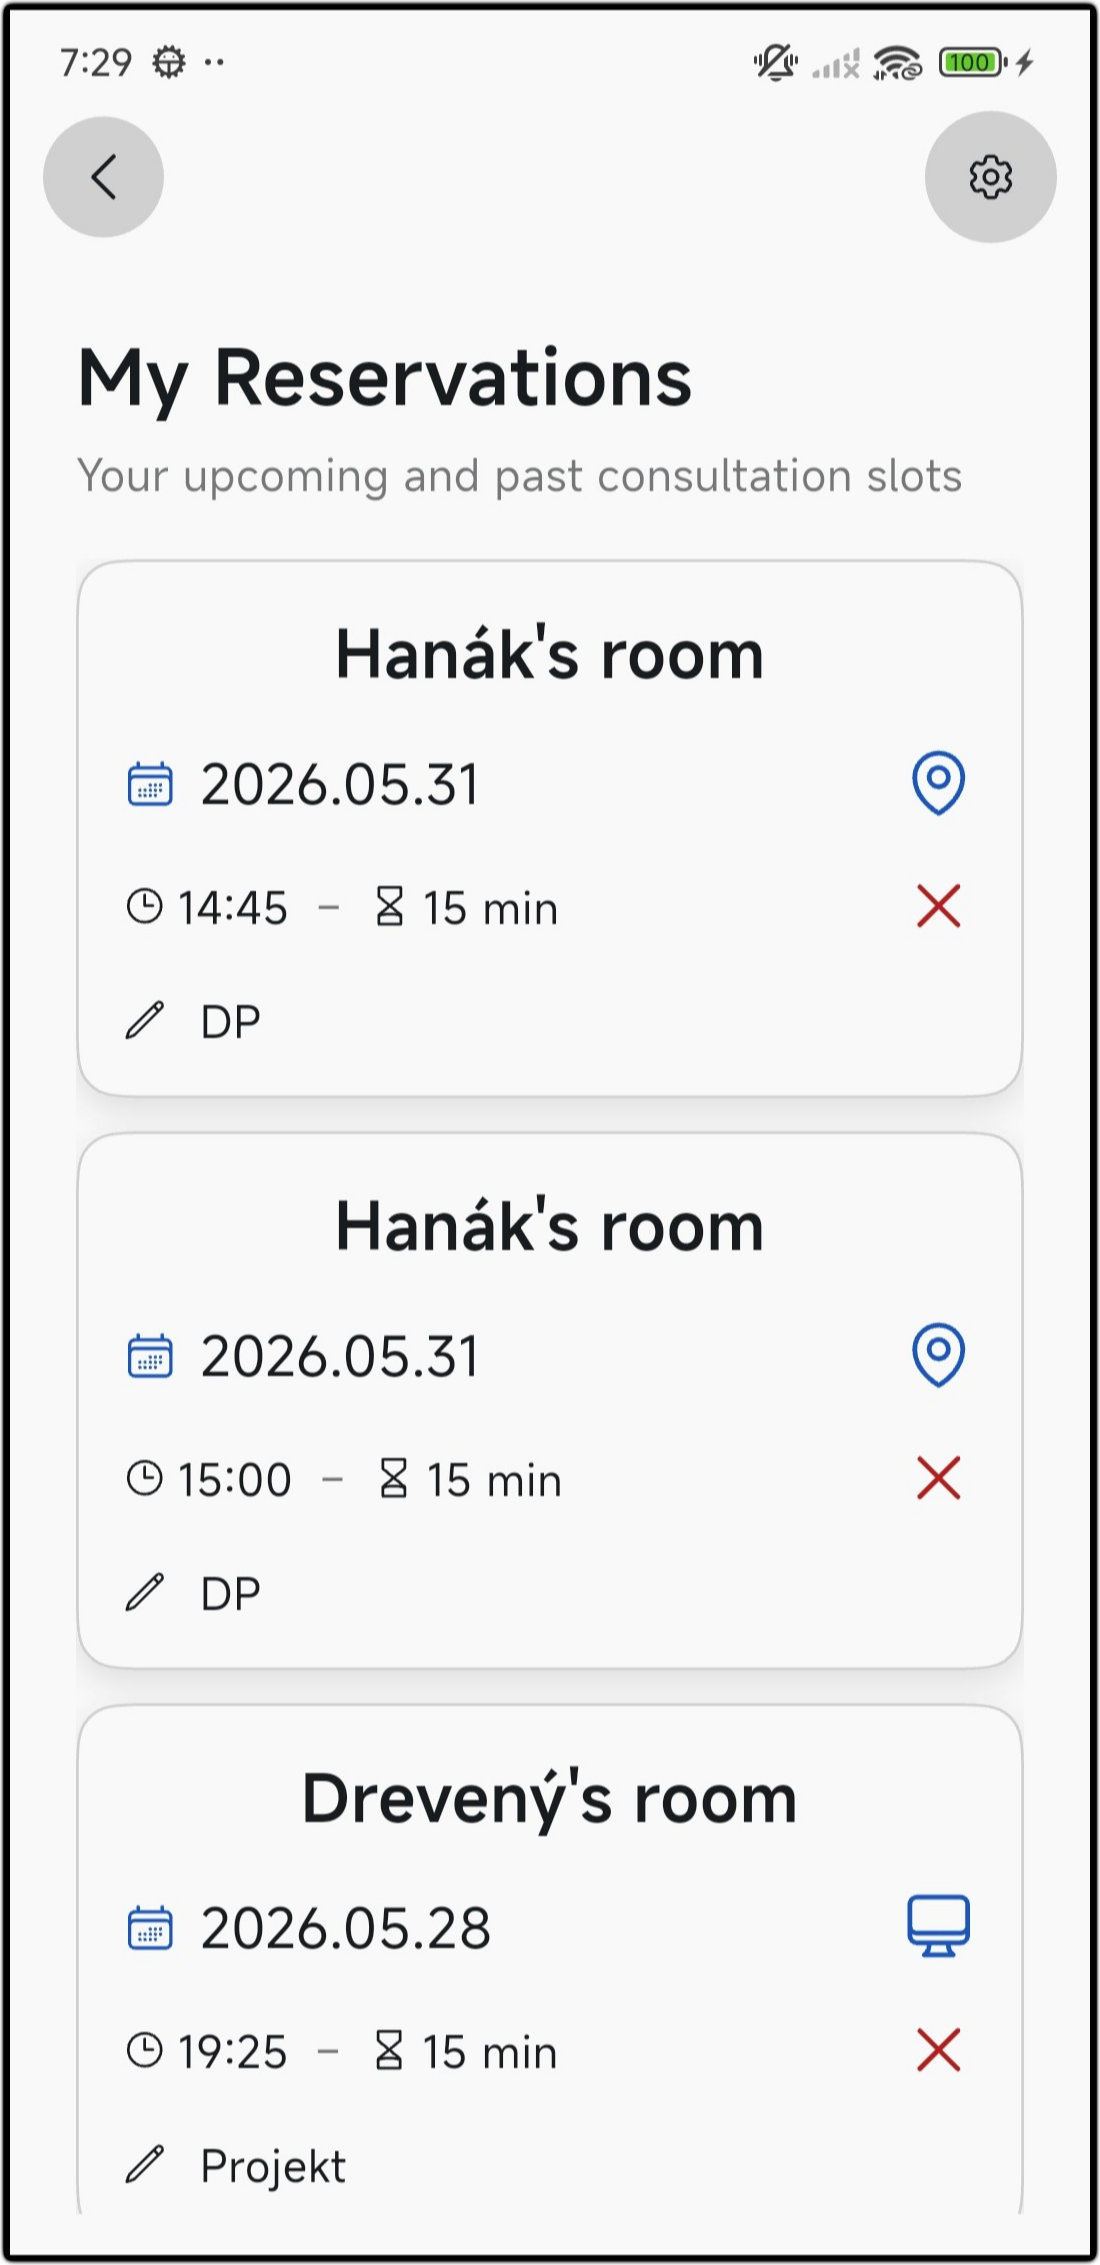
\includegraphics[width=\textwidth]{obrazky-figures/implementacia-my-reservations.png}
    \caption{Obrazovka \textbf{MyReservationsPage} so zoznamom aktívnych rezervácií
    naprieč všetkými miestnosťami. Každá karta zobrazuje názov miestnosti, dátum,
    čas začiatku, trvanie a dôvod návštevy. Ikona polohy alebo obrazovky vpravo hore
    indikuje typ konzultácie a slúži na jeho zmenu. Ikona krížika umožňuje
    okamžité zrušenie rezervácie s optimistickou aktualizáciou UI.}
    \label{fig:my-reservations}
    \end{minipage}
    \hfill
    \begin{minipage}[t]{0.45\textwidth}
        \centering
    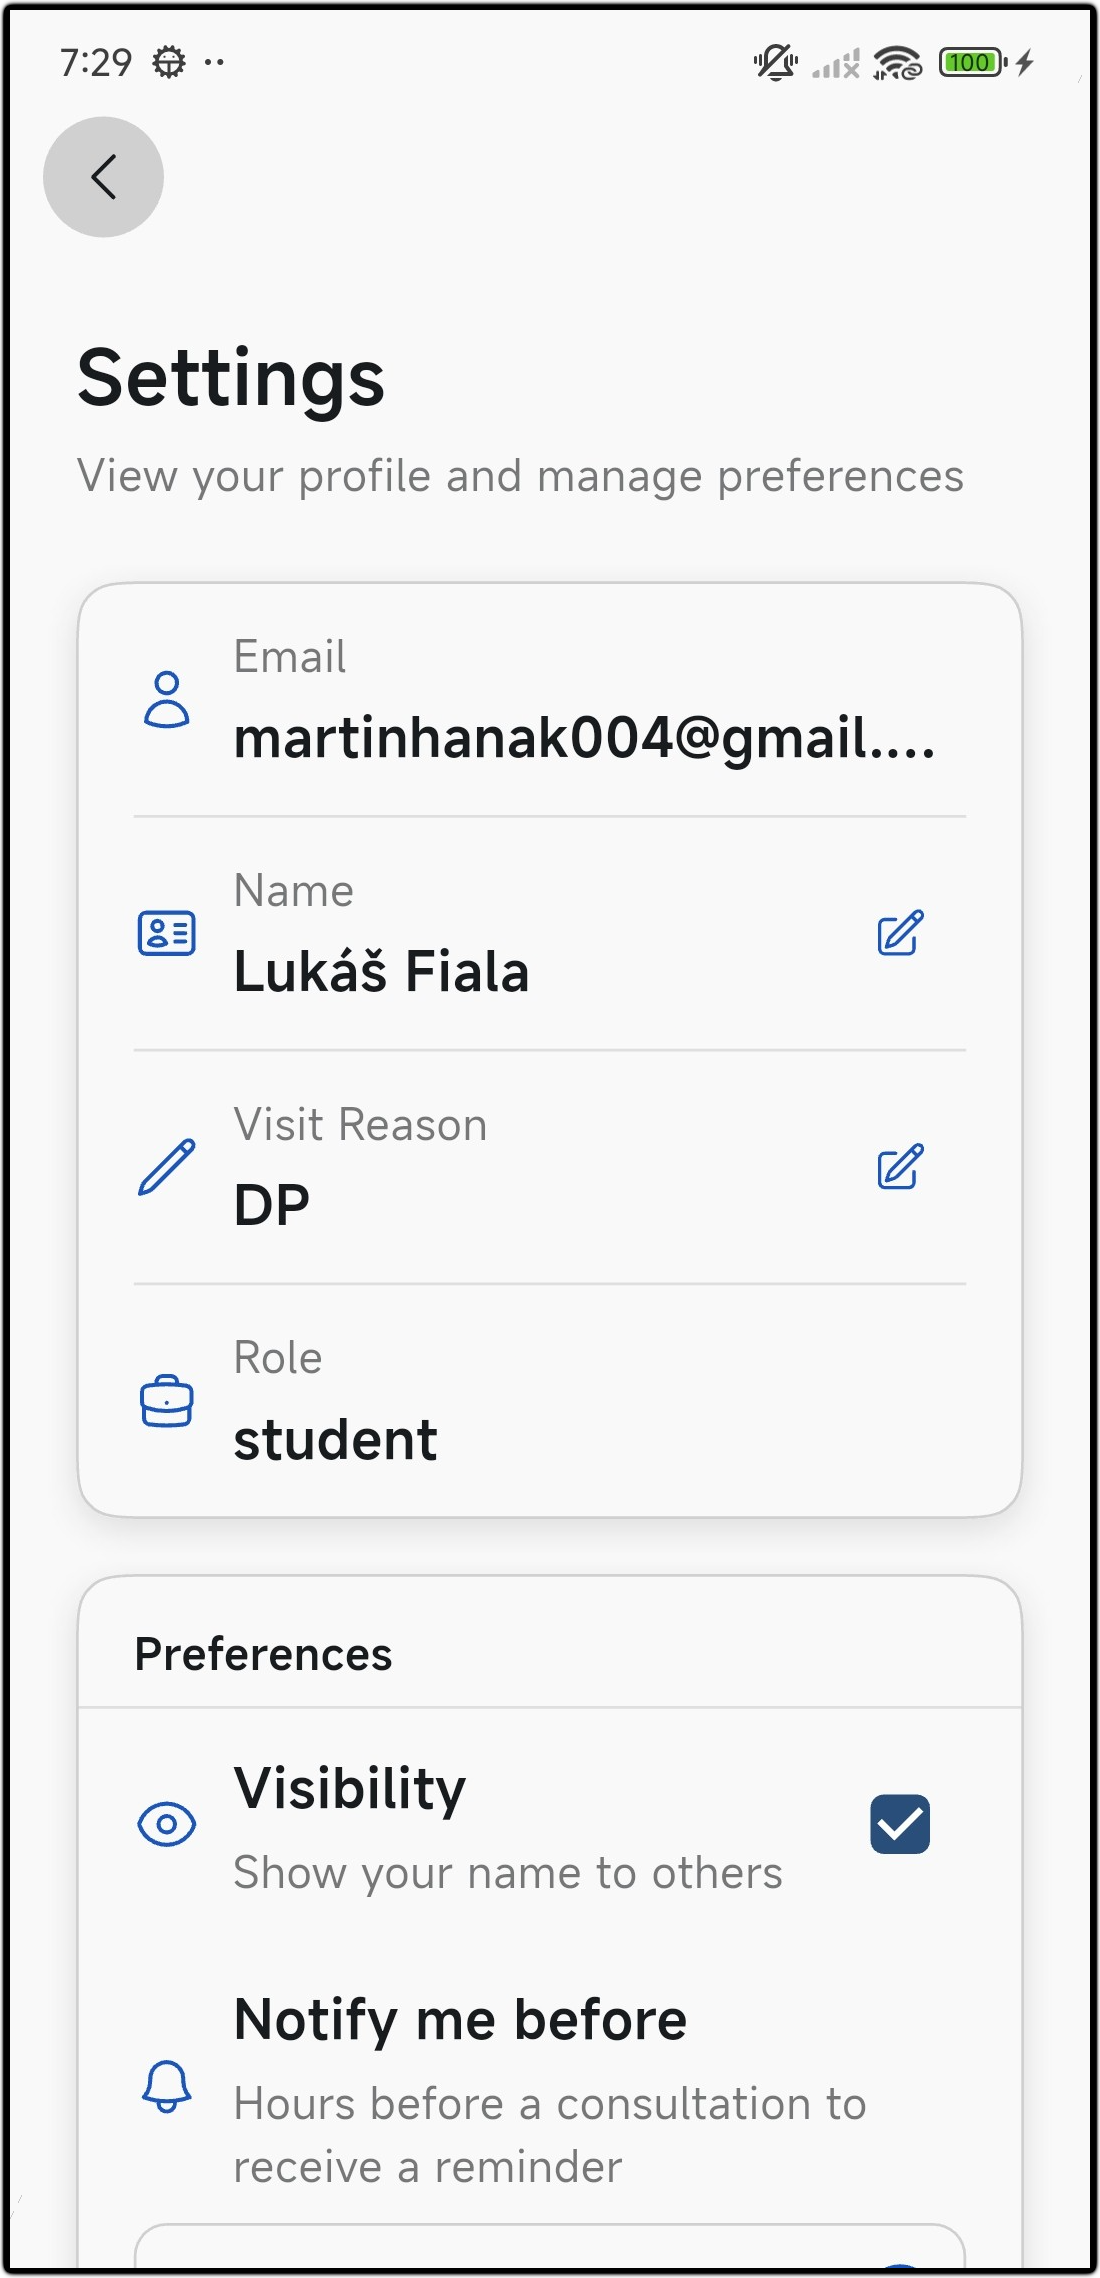
\includegraphics[width=\textwidth]{obrazky-figures/implementacia-settings.png}
    \caption{Obrazovka \textbf{ChangeSettings} zobrazujúca dve z troch kariet.
    Prvá karta obsahuje profilové údaje používateľa: e-mailovú adresu (len na čítanie),
    editovateľné meno cez \textbf{EditableTile} a dôvod návštevy.
    Druhá karta \textit{Preferences} obsahuje prepínač \textbf{Visibility}
    pre GDPR viditeľnosť mena a predvoľbu \textbf{Notify me before}
    pre nastavenie e-mailových upozornení.}
    \label{fig:implementaciasettings}
    \end{minipage}
\end{figure}


\subsection{Obrazovka nastavení (ChangeSettings)}
\label{sec:impl-nastavenia}
Obrazovka nastavení je implementovaná ako \textbf{StatelessWidget}, 
pričom \textbf{ChangeSettings\-ViewModel} sa vytvára kaskádovým volaním 
\textbf{ChangeNotifierProvider(create: (\_ ) => ChangeSettingsViewModel()..initialize())}. 
Metóda \textbf{initialize()} sa teda spustí ihneď po konštrukcii ViewModelu 
a asynchrónne stiahne aktuálne nastavenia používateľa zo servera. 
Kým prebieha načítavanie, obrazovka zobrazuje indikátor načítavania. Po jeho dokončení sa vykreslí pomocný widget \textbf{\_SettingsBody}, 
do ktorého sa deleguje celé rozloženie. Obrazovka je rozčlenená do troch kariet. 

Prvá karta zobrazuje 
\textbf{profil používateľa}: e-mailovú adresu a rolu, ktoré sú iba 
na čítanie a zobrazujú sa pomocou \textbf{InfoTile} a editovateľné 
položky mena, priezviska a dôvodu návštevy (Visit~Reason), 
ku ktorým sa pristupuje cez \textbf{EditableTile}. 
Po klepnutí na ikonu ceruzky sa otvorí príslušný dialóg, 
ktorý po potvrdení zavolá metódu ViewModelu a zmenu synchronizuje so serverom.

Druhá karta obsahuje \textbf{predvoľby}. Prvou z nich je prepínač 
\textbf{Visibility}, ktorý riadi GDPR flag viditeľnosti mena 
voči ostatným používateľom. Tento flag sa prenáša do API pri každej 
jeho zmene cez metódu \textbf{viewModel.setVisibility()} a jeho aktuálna 
hodnota sa zároveň uloží do \textbf{UserPreferences} pre okamžité 
lokálne prekreslenie. Vypnutie viditeľnosti má obojstranný dôsledok – 
používateľ skryje svoje meno ostatným, no ako protiváhu zároveň prestane 
vidieť mená iných používateľov v slotoch. Druhá predvoľba, \textbf{Notify me before}, umožňuje nastaviť,
koľko hodín vopred má systém odoslať e-mailové upozornenie
pred začiatkom rezervovanej konzultácie. Pôvodná implementácia
pracovala s jednou hodnotou, avšak na základe spätnej väzby
od testerov, ktorí požadovali možnosť byť upozornení viackrát
pred tým istým termínom, bola nahradená zoznamom hodnôt.
Predvoľba je implementovaná ako
\textbf{NotifyHoursTile}.
Používateľ zadá počet hodín do číselného vstupného poľa
a hodnotu potvrdí kliknutím na ikonu plus vpravo od poľa,
čím sa zavolá \textbf{viewModel.addNotifyHour(parsed)}.
Takto možno postupne zostaviť zoznam viacerých časových odstupov,
napríklad 24 hodín a 2 hodiny pred konzultáciou.
Aktuálny počet pridaných hodnôt je zobrazený ako odkaz
\textit{View added hours (n)}, ktorý presmeruje na samostatnú
obrazovku so zoznamom, kde je možné jednotlivé záznamy odstrániť
volaním \textbf{viewModel.removeNotifyHour()}. Prázdny zoznam
notifikácie deaktivuje. Každá zmena zoznamu je odoslaná na server volaním \textbf{api.updateNotificationTimes()}
a pri zlyhaní sa zoznam obnoví zo snapshotu pomocou rovnakého
vzoru optimistickej aktualizácie, aký je použitý inde v aplikácii.
Poslednou predvoľbou je \textbf{Theme}: prepínač medzi svetlou 
a tmavou tematikou. Na rozdiel od ostatných nastavení sa táto 
zmena neprenáša na server, ale ukladá výlučne lokálne 
do \textbf{UserPreferences}, pretože ide o čisto vizuálnu preferenciu zariadenia.

Tretia karta, \textbf{Administration}, sa zobrazí podmienene 
len vtedy, keď má ViewModelom načítaná rola hodnotu \textbf{'teacher'}. Obsahuje jedinú akciu 
\textbf{Create Teacher}, ktorá otvorí dialóg pre zadanie e-mailu, 
mena a priezviska nového pedagóga.

\subsection{Znovupoužiteľné komponenty nastavení}
Nastavenia sú oddelené do dvoch 
samostatných súborov: \textbf{settings\_tiles.dart} a \textbf{settings\-\_dialogs.dart}. 


Súbor \textbf{settings\_tiles.dart} definuje päť typov dlaždíc.
\begin{itemize}
    \item \textbf{InfoTile:} Riadok iba na čítanie. Zobrazuje popisok a hodnotu.
    \item \textbf{EditableTile:} Rozširuje \textbf{InfoTile} o ikonu ceruzky, ktorá cez callback \textbf{onEdit} otvorí príslušný dialóg.
    \item \textbf{CheckboxTile:} Riadok s vlastným prepínačom \textbf{CustomCheckbox} 
          vpravo. Ikona sa dynamicky mení podľa aktuálneho stavu 
          (napríklad \textbf{eye\_open}/\textbf{eye\_closed} pre Visibility, 
          \textbf{moon}/\textbf{sun} pre Theme).
          \item \textbf{ActionTile:} Kliknuteľný riadok so šípkou vpravo, 
          určený pre akciu Create~Teacher.
          \item \textbf{NotifyHoursTile:} Jediný \textbf{StatefulWidget}, pretože spravuje vlastný 
          \textbf{TextEditingController} pre číselné vstupné pole. 
          Metóda \textbf{didUpdateWidget} zabezpečuje synchronizáciu 
          poľa s hodnotou ViewModelu v prípade, že sa zmení externe 
          (napríklad po potvrdení zo servera). Ikonka sa mení na preškrtnutú pri hodnote 0.
\end{itemize}

Súbor \textbf{settings\_dialogs.dart} obsahuje tri samostatné 
asynchrónne funkcie – \textbf{showNameDialog}, 
\textbf{showVisitReasonDialog} a \textbf{showCreateTeacherDialog}. 
Dialógy pre editáciu mena a dôvodu návštevy sú implementované 
ako jednoduché \textbf{AlertDialog} widgety so zdieľanými pomocnými 
funkciami \textbf{\_cancelButton} a \textbf{\_saveLabel}, 
čím je zabezpečená vizuálna konzistencia akčných riadkov naprieč 
všetkými dialógmi. Dialóg Create~Teacher navyše využíva 
\textbf{StatefulBuilder} na správu lokálneho stavu načítavania 
a chybovej správy priamo v dialógu bez nutnosti 
povýšenia volajúceho widgetu na \textbf{StatefulWidget}.

\section{Navigácia a prepojenie obrazoviek}
\label{sec:impl-navigacia}
Navigácia v aplikácii je centralizovaná v triede \textbf{NavigationService}, 
ktorá je registrovaná ako singleton prostredníctvom balíčka \textbf{get\_it~\cite{getit}} a sprístupňuje sa globálne cez inštanciu \textbf{nav}. 
Táto trieda obaľuje štandardné metódy Flutteru 
(\textbf{Navigator.push}, \textbf{Navigator.pop}), pričom interne
udržiava \textbf{routeHistory} (zásobník názvov navštívených obrazoviek).
Ten umožňuje \textbf{NavigationService} rozhodnúť, ktorú obrazovku
zobraziť pri stlačení tlačidla späť. Pre každú obrazovku vystavuje pomenovanú navigačnú metódu, 
napríklad \textbf{nav.toCreateBlock(...)}. 
Vďaka tomu nie je v žiadnom ViewModeli ani widgete 
priamo referencovaná žiadna konkrétna trieda obrazovky, 
čo znižuje závislosť medzi vrstvami a uľahčuje prípadné budúce 
zmeny v navigačnom grafe a zároveň robí kód prehľadnejším.

\subsection{AppBar a hamburger menu}
\label{subsec:impl-appbar}
Obrazovky aplikácie využívajú zdieľaný widget \textbf{AppBarMenu} 
ako hodnotu parametra \textbf{appBar} v \textbf{Scaffold}. 
Jeho obsah sa mení podľa kontextu: na hlavných obrazovkách
sa vpravo zobrazuje ikona s tromi čiarami, otvárajúca bočné menu \textbf{SliderMenu} s navigačnými položkami, zatiaľ čo na vnorených obrazovkách je nahradená šípkou späť volajúcou \textbf{nav.pop()}.
V strede AppBaru sa na hlavnej obrazovke Majiteľa nachádza
prepínač \textbf{AnimatedToggle} pre prepínanie medzi rolami a odkaz na nastavenia je zobrazený len na obrazovkách, kde to je relevantné. Na samotnej stránke nastavení sa vďaka parametru \textbf{onSettingsPage: true} skryje.

\subsection{Navigačné metódy a spätné volanie onSuccess}
\label{subsec:implonsuccess}
Na niektorých obrazovkách sa používa vzor
odovzdania callbacku \textbf{onSuccess}. Každá takáto obrazovka deklaruje parameter \textbf{final VoidCallback? onSuccess}
a po úspešnom dokončení operácie ho zavolá ešte pred \textbf{nav.pop()}.
Napríklad \textbf{AddSlotPage} (obrázok~\ref{fig:create-slot}) má signatúru:
\begin{minted}{dart}
class AddSlotPage extends StatefulWidget {
  final int blockId;
  final VoidCallback? onSuccess;
  ...
}
\end{minted}
\noindent a pri navigácii rodič odovzdá vlastnú metódu ViewModelu:
\begin{minted}{dart}
nav.toAddSlot(
  blockId: widget.blockId,
  onSuccess: () => viewModel.refetchData(widget.blockId),
);
\end{minted}
Keď potomok zavolá \textbf{widget.onSuccess?.call()} ešte pred
\textbf{nav.pop()}, rodič si znovunačíta dáta zo servera skôr,
ako sa obrazovka zobrazí. Návrat je teda vždy do aktuálneho stavu, napríklad \textbf{viewModel.loadRoom()} pri prechode na
\textbf{CreateBlockPage} alebo \textbf{EditBlockPage}, alebo
\textbf{viewModel.refetchData(blockId)} pri prechode na \textbf{AddSlotPage}.

\section{Znovupoužiteľné widgety a vizuálne prvky}
\label{sec:impl-custom-widgets}

Táto sekcia opisuje widgety zdieľané naprieč viacerými obrazovkami aplikácie,
rozdelené podľa adresárovej štruktúry.

\subsubsection{Priečinok custom\_widgets/}
\begin{itemize}
    \item \textbf{AnimatedToggle:} Animovaný prepínač s \textit{pill} animáciou. Používa sa na prepínanie medzi rolami Majiteľa a Návštevníka.
    \item \textbf{AppBarMenu:} Zdieľaný panel implementovaný ako \textbf{PreferredSizeWidget}. Podľa kontextu zobrazuje hamburger alebo šípku späť, ikonu nastavení a voliteľný \textbf{AnimatedToggle}.
    \item \textbf{SliderMenu:} Bočné menu odovzdávané do parametra \textbf{drawer}. Dáta načítava cez vlastný \textbf{SliderMenuViewModel}. Položka Create Room je viditeľná len pre Majiteľa.
    \item \textbf{CustomInputTextField:} Konfigurovateľné textové pole so vstavanou správou životného cyklu kontroléra a podporou typov \textbf{text}, \textbf{email}, \textbf{url} a \textbf{number}.
    \item \textbf{CustomDateRangePickerDialog:} Dialóg pre výber dátumov s režimami \textit{multiple} a \textit{range}. Používa sa pri vytváraní a kopírovaní blokov.
    \item \textbf{CustomTimeDurationPicker:} Dvojica \textbf{CupertinoPicker} komponentov pre výber trvania slotu a času začiatku. Používa sa na obrazovke \textbf{CreateBlockPage} a \textbf{AddSlotPage}.
    \item \textbf{RoomFormBody:} Zdieľaný formulár pre \textbf{CreateRoomPage} a \textbf{EditRoomPage} prijímajúci ViewModel typovaný ako \textbf{BaseRoomViewModel}.
    \item \textbf{CustomCheckbox:} Obal nad štandardným \textbf{Checkbox} widgetom so zväčšením dotykovej plochy o~20~\%.
\end{itemize}

\subsubsection{Priečinok base\_consultations/}
\textbf{RoomSelectorButton} zabezpečuje výber aktívnej miestnosti a zostáva prilepený
k vrchu obrazovky pri skrolovaní pomocou \textbf{StickyHeader}. \textbf{NoRoomsFound} zobrazuje prispôsobenú správu a akciu podľa roly. Widgety
\textbf{ConsultationBlockCard} a \textbf{ConsultationsContent} sú opísané
v sekcii~\ref{subsec:bloky-sloty}.

\subsubsection{Priečinok slots/}
Hlavné widgety slotov (\textbf{SlotWidget}, \textbf{FreeSlot}, \textbf{CurrentUserSlot},
\textbf{AnotherUsersSlot}, \textbf{TakeSlotBottomSheet}, \textbf{TypeBottomSheet})
sú opísané v sekcii~\ref{subsec:bloky-sloty}. \textbf{TypeBottomSheet} umožňuje
zmenu typu konzultácie (online\,/\,osobne) bez potreby zrušenia rezervácie. Pomocné widgety zahŕňajú
\textbf{SlotTime} pre zobrazenie času a trvania, prepínač stavu \textbf{TypeToggle} a \textbf{KeyboardPadding} pre priestor pri zobrazenej klávesnici.

\subsubsection{Priečinok settings/}
Widgety v tomto priečinku sú opísané v sekcii~\ref{sec:impl-nastavenia}.